\documentclass{beamer}

\usepackage[T1]{fontenc}
\usepackage[utf8]{inputenc}
\usepackage{amsmath,amssymb,amsfonts,amsthm}
\usepackage{physics}
\usepackage{bm}
\usepackage{mathtools}
% indicator function via \mathbf{1}
\usepackage{tikz}
\usetikzlibrary{quantikz,arrows.meta,positioning,decorations.pathreplacing}
\usepackage{listings}
\usepackage{xcolor}

% Python listing style
\lstset{
  language=Python,
  basicstyle=\ttfamily\tiny,
  keywordstyle=\color{blue!80!black}\bfseries,
  commentstyle=\color{green!50!black}\itshape,
  stringstyle=\color{red!60!black},
  numberstyle=\tiny\color{gray},
  numbers=left,
  stepnumber=5,
  numbersep=4pt,
  backgroundcolor=\color{gray!8},
  showstringspaces=false,
  breaklines=true,
  frame=single,
  rulecolor=\color{gray!50},
  tabsize=4,
  captionpos=b
}

% ---- tightened beamer spacing ----
\setlength{\jot}{4pt}

\title{The Quantum Approximate Optimization Algorithm (QAOA)}
\subtitle{From Foundations to Gradient Methods}
\author{Morten Hjorth-Jensen}
\date{Spring 2026}

\begin{document}

\frame{\titlepage}

%------------------------------------------------
\begin{frame}{Outline}
\tableofcontents
\end{frame}


\begin{frame}[plain,fragile]
\frametitle{Plans for the week of April 20-24, 2026}

\begin{block}{}
\begin{enumerate}
 \item The Quantum Approximate Optimization Algorithm (QAOA), theory and code examples
 \item Short introduction to Quantum Support Vector Machine Learning (QSVM), if we get time

% \item Video of lecture at \href{{https://youtu.be/C36Kg4eaO7A}}{\nolinkurl{https://youtu.be/C36Kg4eaO7A}}

% \item Whiteboard notes at \href{{https://github.com/CompPhysics/QuantumComputingMachineLearning/blob/gh-pages/doc/HandWrittenNotes/2\
%025/NotesApril23.pdf}}{\nolinkurl{https://github.com/CompPhysics/QuantumComputingMachineLearning/blob/gh-pages/doc/HandWrittenNotes/2\
%025/NotesApril23.pdf}}
\end{enumerate}

\noindent
\end{block}


%================================================
\section{Combinatorial Optimization and QUBO}
%================================================

\begin{frame}{Combinatorial Optimization: Problem Setting}
Let $\mathbf{x} = (x_1,\dots,x_n)\in\{0,1\}^n$ be a binary decision
vector. The general \textbf{combinatorial optimization} task is
\[
\mathbf{x}^* \;=\; \arg\min_{\mathbf{x}\in\{0,1\}^n} C(\mathbf{x}),
\]
where $C:\{0,1\}^n\to\mathbb{R}$ is a cost function.

\medskip

The search space has $2^n$ elements — exponential in $n$.

\medskip

\textbf{Complexity classes:}
\begin{itemize}
\item Problems in \textbf{P} can be solved in polynomial time.
\item Most interesting instances are \textbf{NP-hard}: no known
  polynomial-time algorithm exists.
\end{itemize}

\textbf{Approximation goal.}  Find $\mathbf{x}$ achieving
\[
\alpha \;=\; \frac{C(\mathbf{x}^*)}{C_{\min}} \;\lesssim\; 1,
\]
where $\alpha$ is the \emph{approximation ratio}.
\end{frame}

%------------------------------------------------

\begin{frame}{QUBO: Rigorous Formulation}
\textbf{Definition (QUBO).}  A \emph{Quadratic Unconstrained Binary
Optimization} problem is specified by a real, symmetric matrix
$Q\in\mathbb{R}^{n\times n}$ and the objective
\[
\boxed{
C_Q(\mathbf{x}) \;=\; \mathbf{x}^T Q\,\mathbf{x}
\;=\; \sum_{i=1}^n Q_{ii}\,x_i
\;+\; \sum_{i<j}(Q_{ij}+Q_{ji})\,x_i x_j,}
\]
where $x_i\in\{0,1\}$.

Key properties:
\begin{itemize}
\item Because $x_i^2 = x_i$ for binary variables, all diagonal and
  off-diagonal terms contribute.
\item Any polynomial objective over binary variables can be
  \emph{reduced} to QUBO by degree reduction.
\item QUBO is NP-hard in general (contains 3-SAT as a special case).
\end{itemize}
\end{frame}

%------------------------------------------------

\begin{frame}{QUBO to Ising: Variable Substitution}
The \textbf{Ising substitution} replaces binary variables
$x_i\in\{0,1\}$ with spin variables $s_i\in\{-1,+1\}$:
\[
x_i = \frac{1 - s_i}{2}
\qquad\Longleftrightarrow\qquad
s_i = 1 - 2x_i.
\]

Substituting into the QUBO objective:
\begin{align*}
C_Q(\mathbf{x})
&= \sum_{i<j}(Q_{ij}+Q_{ji})
   \frac{(1-s_i)}{2}\frac{(1-s_j)}{2}
   + \sum_i Q_{ii}\frac{(1-s_i)}{2}\\[4pt]
&= \underbrace{\sum_{i<j} \frac{Q_{ij}+Q_{ji}}{4}\,s_i s_j}_{J_{ij}\,s_i s_j\text{ coupling}}
   + \underbrace{\sum_i \left(-\frac{Q_{ii}}{2}
   - \sum_{j\neq i}\frac{Q_{ij}+Q_{ji}}{4}\right)s_i}_{h_i\,s_i\text{ field}}
   + \text{const.}
\end{align*}

So any QUBO is equivalent to an \textbf{Ising model}
$\mathcal{H}(\mathbf{s}) = \sum_{i<j}J_{ij}s_is_j + \sum_i h_i s_i$.
\end{frame}

%------------------------------------------------

\begin{frame}{Ising Model as a Quantum Hamiltonian}
Promote the classical spin variables $s_i\in\{-1,+1\}$ to
\textbf{Pauli-$Z$ operators} $Z_i$ acting on qubit $i$:

\[
Z_i \;=\; \begin{pmatrix}1&0\\0&-1\end{pmatrix}_i,\qquad
Z_i\ket{0} = \ket{0},\quad Z_i\ket{1}=-\ket{1}.
\]

The computational basis states $\ket{\mathbf{z}} =
\ket{z_1,\dots,z_n}$ with $z_i\in\{0,1\}$ are simultaneous
eigenstates of all $Z_i$ with eigenvalue $(-1)^{z_i}$.

\medskip

The \textbf{cost Hamiltonian} is the quantum version of the Ising energy:
\[
\boxed{
H_C \;=\; \sum_{i<j} J_{ij}\,Z_i Z_j \;+\; \sum_i h_i\,Z_i.}
\]

It is diagonal in the computational basis:
\[
H_C\ket{\mathbf{z}} \;=\; \mathcal{H}(\mathbf{z})\,\ket{\mathbf{z}},
\qquad \mathcal{H}(\mathbf{z}) = C(\mathbf{z}),
\]
so the ground state of $H_C$ encodes the optimal solution.
\end{frame}

%------------------------------------------------

\begin{frame}{QUBO to Ising: Explicit Coefficient Map}
Given $Q\in\mathbb{R}^{n\times n}$ symmetric, the Ising coefficients are:

\medskip

\begin{center}
\begin{tabular}{lll}
\hline
\textbf{Ising coefficient} & \textbf{Formula} & \textbf{Origin} \\
\hline
$J_{ij}$, $i<j$ &
$\dfrac{Q_{ij}+Q_{ji}}{4} = \dfrac{Q_{ij}}{2}$ &
$x_ix_j \to \tfrac{1}{4}(1-s_i)(1-s_j)$\\[8pt]
$h_i$ &
$-\dfrac{Q_{ii}}{2} - \displaystyle\sum_{j\neq i}\frac{Q_{ij}}{2}$ &
linear terms after substitution \\[8pt]
constant & $\displaystyle\frac{1}{4}\sum_{i,j}Q_{ij}$ & absorbed into energy offset \\
\hline
\end{tabular}
\end{center}

\medskip

\textbf{Key point:} minimizing $C_Q(\mathbf{x})$ over
$\{0,1\}^n$ is \emph{identical} to finding the ground state of $H_C$
over $\{-1,+1\}^n$, shifted by the constant.
\end{frame}

%------------------------------------------------

\begin{frame}{QUBO to Ising: Worked Numerical Example}
Take $n=2$ with $Q = \begin{pmatrix}1 & -2\\ -2 & 1\end{pmatrix}$,
so $C_Q(x_1,x_2) = x_1 - 4x_1x_2 + x_2$.

\medskip
\textbf{Reading off the Ising coefficients} via $J_{12}=(Q_{12}+Q_{21})/4$,
$h_i = -Q_{ii}/2 - \sum_{j\neq i}Q_{ij}/2$:
\[
J_{12} = \tfrac{-2+(-2)}{4} = -1,\quad
h_1 = -\tfrac{1}{2}-\tfrac{-2}{2} = \tfrac{1}{2},\quad
h_2 = \tfrac{1}{2},\quad
\text{const} = \tfrac{1-2-2+1}{4} = -\tfrac{1}{2}.
\]
\textbf{Hamiltonian:}
$H_C = -Z_1Z_2 + \tfrac{1}{2}Z_1 + \tfrac{1}{2}Z_2$.

\medskip
\textbf{Verification} against $C_Q - \text{const}$ for all four bitstrings:
\begin{center}
\small
\begin{tabular}{cccccc}
\hline
$\mathbf{x}$ & $C_Q$ & $\mathbf{s}=(1-2\mathbf{x})$ & $\mathcal{H}(\mathbf{s})=J_{12}s_1s_2+h_1s_1+h_2s_2$ & $C_Q-\text{const}$ \\
\hline
$(0,0)$ & $0$  & $(+1,+1)$ & $-1+\tfrac{1}{2}+\tfrac{1}{2}=0$ & $0+\tfrac{1}{2}=\tfrac{1}{2}$ \\
$(0,1)$ & $1$  & $(+1,-1)$ & $+1+\tfrac{1}{2}-\tfrac{1}{2}=1$ & $1+\tfrac{1}{2}=\tfrac{3}{2}$ \\
$(1,0)$ & $1$  & $(-1,+1)$ & $+1-\tfrac{1}{2}+\tfrac{1}{2}=1$ & $1+\tfrac{1}{2}=\tfrac{3}{2}$ \\
$(1,1)$ & $-2$ & $(-1,-1)$ & $-1-\tfrac{1}{2}-\tfrac{1}{2}=-2$ & $-2+\tfrac{1}{2}=-\tfrac{3}{2}$ \\
\hline
\end{tabular}
\end{center}
$\mathcal{H}(\mathbf{s}) = C_Q(\mathbf{x}) - \text{const}$. \checkmark\quad
Ground state: $\mathbf{x}^*=(1,1)$, $C_Q^{\min}=-2$.
\end{frame}

%------------------------------------------------

\begin{frame}{MaxCut Problem: Definition}
\textbf{Definition (MaxCut).}  Given an undirected weighted graph
$G = (V,E,\mathbf{w})$ with $|V|=n$ vertices and edge weights
$w_{ij}>0$, find a partition $V = S \cup \bar{S}$ that
\textbf{maximizes} the total weight of cut edges:
\[
\text{MaxCut}(S) \;=\; \sum_{(i,j)\in E} w_{ij}\,
\mathbf{1}[i\in S,\,j\notin S].
\]

\medskip

In binary variables: assign $x_i = 1$ if $i\in S$, $x_i=0$ otherwise.
An edge $(i,j)$ is cut iff $x_i \neq x_j$, i.e., $x_i(1-x_j) +
(1-x_i)x_j = x_i + x_j - 2x_ix_j$. So:
\[
C_{\rm MC}(\mathbf{x}) \;=\;
\sum_{(i,j)\in E} w_{ij}\,(x_i + x_j - 2x_ix_j).
\]

\textbf{MaxCut is NP-hard} (Garey \& Johnson, 1979). Best classical
approximation: Goemans--Williamson SDP gives ratio $\alpha \ge 0.878$.
\end{frame}

%------------------------------------------------

\begin{frame}{MaxCut: Full QUBO Derivation}
Starting from $C_{\rm MC} = \sum_{(i,j)\in E}w_{ij}(x_i+x_j-2x_ix_j)$,
write in matrix form. Define the QUBO matrix $Q$ with:
\[
Q_{ij} = \begin{cases}
-2w_{ij} & \text{if }(i,j)\in E \\
\sum_{k:(i,k)\in E} w_{ik} & \text{if } i=j \\
0 & \text{otherwise.}
\end{cases}
\]

Then $C_{\rm MC}(\mathbf{x}) = \mathbf{x}^T Q\,\mathbf{x}$.

\medskip

More compactly, note that $x_i(1-x_j)$ is a valid QUBO term.
It is conventional to write
\[
C_{\rm MC}(\mathbf{x}) \;=\; \sum_{(i,j)\in E} w_{ij}\,x_i(1-x_j)
\;+\; \text{symmetric counterpart}
\;=\;\sum_{(i,j)\in E} w_{ij}(x_i + x_j - 2x_ix_j).
\]
\end{frame}

%------------------------------------------------

\begin{frame}{MaxCut: QUBO $\to$ Ising $\to$ Pauli Operator}
\textbf{Step 1: Ising substitution.} Set $x_i = (1-s_i)/2$. Then
$x_i + x_j - 2x_ix_j = \tfrac{1}{2}(1 - s_is_j)$, so
\[
C_{\rm MC}(\mathbf{s}) \;=\;
\sum_{(i,j)\in E} w_{ij}\,\frac{1-s_is_j}{2}
\;=\; \frac{1}{2}\sum_{(i,j)\in E}w_{ij}
\;-\; \frac{1}{2}\sum_{(i,j)\in E}w_{ij}\,s_is_j.
\]

\textbf{Step 2: Promote to operators.} Replace $s_i \to Z_i$:
\[
\boxed{
H_C^{\rm MC} \;=\; \frac{1}{2}\sum_{(i,j)\in E} w_{ij}(I - Z_iZ_j).}
\]

Verification: $H_C^{\rm MC}\ket{\mathbf{z}} = C_{\rm MC}(\mathbf{z})\ket{\mathbf{z}}$.

For unit weights ($w_{ij}=1$):
\[
H_C^{\rm MC} \;=\; \frac{|E|}{2}\,I \;-\; \frac{1}{2}\sum_{(i,j)\in E}Z_iZ_j.
\]

\textbf{Maximizing $C_{\rm MC}$ = minimizing $-H_C^{\rm MC}$ = finding
the ground state.}
\end{frame}

%------------------------------------------------

\begin{frame}{MaxCut: Example on a 4-Cycle Graph}
\begin{columns}
\begin{column}{0.35\textwidth}
\centering
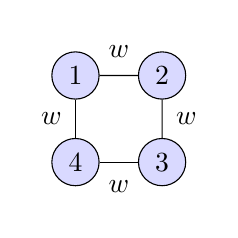
\begin{tikzpicture}[scale=1.1,every node/.style={circle,draw,fill=blue!15,
  minimum size=6mm,inner sep=1pt}]
\node (1) at (0,1)  {1};
\node (2) at (1,1)  {2};
\node (3) at (1,0)  {3};
\node (4) at (0,0)  {4};
\draw (1)--(2) node[midway,above,draw=none,fill=none]{$w$};
\draw (2)--(3) node[midway,right,draw=none,fill=none]{$w$};
\draw (3)--(4) node[midway,below,draw=none,fill=none]{$w$};
\draw (4)--(1) node[midway,left,draw=none,fill=none]{$w$};
\end{tikzpicture}
\end{column}
\begin{column}{0.6\textwidth}
For $G = C_4$ with unit weights:
\[
H_C = \frac{1}{2}
\bigl(
4I - Z_1Z_2 - Z_2Z_3 - Z_3Z_4 - Z_4Z_1
\bigr).
\]

Optimal cut: $S=\{1,3\}$, $\bar S=\{2,4\}$.

Bitstring: $\mathbf{z}=(1,0,1,0)$, giving $C_{\rm MC}=4=|E|$.

\medskip
$H_C\ket{1010} = 4\ket{1010}$ \checkmark
\end{column}
\end{columns}
\end{frame}


%================================================
\section{Variational Quantum Algorithms}
%================================================

\begin{frame}{The Variational Principle for Quantum Optimization}
Any Hamiltonian $H_C$ satisfies the \textbf{variational bound}:
\[
\langle\psi|H_C|\psi\rangle \;\ge\; E_{\min}
\qquad\forall\,|\psi\rangle,
\]
with equality iff $|\psi\rangle$ is the ground state.

\medskip

For optimization we want to \emph{maximize} $\langle H_C \rangle$
(since MaxCut is a maximization problem), so:
\[
\max_{|\psi\rangle}\langle\psi|H_C|\psi\rangle \;=\; E_{\max}.
\]

\textbf{Idea (VQA):} Restrict to a parameterized family
$\{|\psi(\boldsymbol{\theta})\rangle\}$
and optimize over $\boldsymbol{\theta}$ classically:
\[
\boldsymbol{\theta}^* = \arg\max_{\boldsymbol{\theta}}
\underbrace{\langle\psi(\boldsymbol{\theta})|H_C|\psi(\boldsymbol{\theta})\rangle}_{=:\,E(\boldsymbol{\theta})}.
\]
\end{frame}

%------------------------------------------------

\begin{frame}{VQE and the Hybrid Loop}
The \textbf{Variational Quantum Eigensolver (VQE)} implements:

\begin{enumerate}
\item Prepare $|\psi(\boldsymbol{\theta})\rangle = U(\boldsymbol{\theta})|0\rangle^{\otimes n}$
  on the quantum device.
\item Decompose $H_C = \sum_\alpha h_\alpha P_\alpha$ into Pauli strings.
\item Measure each expectation value
  $\langle P_\alpha\rangle = \langle\psi|P_\alpha|\psi\rangle$.
\item Form $E(\boldsymbol{\theta}) = \sum_\alpha h_\alpha \langle P_\alpha\rangle$.
\item Update $\boldsymbol{\theta}$ via a classical optimizer; go to step 1.
\end{enumerate}

\medskip

\textbf{QAOA} is VQE with a \emph{problem-specific} ansatz
$U(\boldsymbol{\gamma},\boldsymbol{\beta})$ determined entirely by
$H_C$ and $H_M$, rather than an ad hoc parameterized circuit.
\end{frame}


%================================================
\section{QAOA: Definition and Hamiltonians}
%================================================

\begin{frame}{The Mixing Hamiltonian}
The \textbf{mixing (driver) Hamiltonian} is
\[
H_M \;=\; \sum_{i=1}^n X_i, \qquad
X_i = \begin{pmatrix}0&1\\1&0\end{pmatrix}_i.
\]

Properties:
\begin{itemize}
\item $H_M$ does \emph{not} commute with $H_C$ (which is diagonal in
  $Z$-basis), so it generates non-trivial transitions.
\item Its ground state is $|+\rangle^{\otimes n} =
  (|0\rangle+|1\rangle)^{\otimes n}/2^{n/2}$, the equal
  superposition state.
\item The unitary $e^{-i\beta H_M} = \bigotimes_i e^{-i\beta X_i} =
  \bigotimes_i R_x(2\beta)$ is a product of single-qubit rotations,
  hence easy to implement.
\end{itemize}

Alternative choices include XY mixers (for constrained problems) and
Grover mixers, but the transverse-field $\sum X_i$ is standard.
\end{frame}

%------------------------------------------------

\begin{frame}{QAOA: Formal Definition}
\textbf{Definition (QAOA).} Given $H_C$ and $H_M$, the depth-$p$ QAOA state is
\[
\boxed{
|\psi_p(\boldsymbol{\gamma},\boldsymbol{\beta})\rangle
\;=\;
\prod_{k=1}^{p}
\underbrace{e^{-i\beta_k H_M}}_{U_M(\beta_k)}
\underbrace{e^{-i\gamma_k H_C}}_{U_C(\gamma_k)}
\;|\!+\rangle^{\otimes n},}
\]
with variational parameters
$\boldsymbol{\gamma}=(\gamma_1,\dots,\gamma_p)\in[0,2\pi)^p$ and
$\boldsymbol{\beta}=(\beta_1,\dots,\beta_p)\in[0,\pi)^p$.

\medskip

The \textbf{variational objective} is
\[
F_p(\boldsymbol{\gamma},\boldsymbol{\beta})
\;=\; \langle\psi_p|H_C|\psi_p\rangle,
\qquad
(\boldsymbol{\gamma}^*,\boldsymbol{\beta}^*)
= \arg\max F_p,
\qquad
\alpha = \frac{F_p^*}{C_{\max}}.
\]

\textbf{Claim (Farhi et al.\ 2014):} $F_p \to C_{\max}$ as $p\to\infty$.
\end{frame}

%------------------------------------------------

\begin{frame}{Initial State}
The initial state is the uniform superposition:
\[
|\!+\rangle^{\otimes n}
\;=\; H^{\otimes n}|0\rangle^{\otimes n}
\;=\; \frac{1}{2^{n/2}}\sum_{\mathbf{z}\in\{0,1\}^n}|\mathbf{z}\rangle.
\]

\medskip

Two complementary interpretations:
\begin{itemize}
\item \textbf{Algorithmic:} represents complete ignorance about the
  solution; all $2^n$ candidates have equal amplitude.
\item \textbf{Physical:} ground state of $-H_M = -\sum_i X_i$,
  so the system starts in the ground state of the driver and then
  gets adiabatically guided toward the ground state of $H_C$.
\end{itemize}

\medskip

Preparation cost: $n$ Hadamard gates.
\end{frame}

%------------------------------------------------

\begin{frame}{Cost Unitary: Explicit Action}
The cost unitary $U_C(\gamma) = e^{-i\gamma H_C}$ is diagonal in the
computational basis. Because $H_C|\mathbf{z}\rangle = C(\mathbf{z})|\mathbf{z}\rangle$:
\[
U_C(\gamma)|\mathbf{z}\rangle
\;=\; e^{-i\gamma C(\mathbf{z})}|\mathbf{z}\rangle.
\]

Acting on a superposition:
\[
U_C(\gamma)\sum_{\mathbf{z}}\alpha_{\mathbf{z}}|\mathbf{z}\rangle
\;=\; \sum_{\mathbf{z}}\alpha_{\mathbf{z}}\,e^{-i\gamma C(\mathbf{z})}|\mathbf{z}\rangle.
\]

\textbf{Interpretation:} $U_C$ applies a phase $e^{-i\gamma C(\mathbf{z})}$
proportional to the cost to each basis state. High-cost strings
acquire more phase, which quantum interference later converts into
amplitude.

\medskip

For $H_C = \sum_{(i,j)\in E}w_{ij}(I-Z_iZ_j)/2$:
\[
U_C(\gamma) = \prod_{(i,j)\in E}
e^{-i\gamma w_{ij}(I-Z_iZ_j)/2}
= e^{-i\gamma \sum_{ij}w_{ij}/2}
\prod_{(i,j)\in E}e^{i\gamma w_{ij}Z_iZ_j/2}.
\]
\end{frame}

%------------------------------------------------

\begin{frame}{Mixer Unitary: Explicit Action}
The mixer unitary $U_M(\beta) = e^{-i\beta H_M}$ factorizes:
\[
U_M(\beta)
\;=\; \bigotimes_{i=1}^n e^{-i\beta X_i}
\;=\; \bigotimes_{i=1}^n R_x(2\beta).
\]

Using $X_i^2 = I$ and the Euler formula:
\[
e^{-i\beta X_i}
= \cos\beta\,I - i\sin\beta\,X_i
= \begin{pmatrix}\cos\beta & -i\sin\beta \\ -i\sin\beta & \cos\beta\end{pmatrix}.
\]

Its action on a single qubit:
\[
e^{-i\beta X}|0\rangle = \cos\beta|0\rangle - i\sin\beta|1\rangle,
\qquad
e^{-i\beta X}|1\rangle = -i\sin\beta|0\rangle + \cos\beta|1\rangle.
\]

$U_M$ \textbf{rotates} every qubit around the $x$-axis, mixing
$|0\rangle$ and $|1\rangle$ amplitudes across all $2^n$ basis states.
\end{frame}


%================================================
\section{Adiabatic Origins and Trotterization}
%================================================

\begin{frame}{Quantum Adiabatic Algorithm (QAA)}
The \textbf{Quantum Adiabatic Algorithm} (Farhi et al.\ 2000) solves
optimization by slowly evolving under
\[
H(s) \;=\; (1-s)\,H_M + s\,H_C, \qquad s \in [0,1],\quad s = t/T.
\]

\textbf{Adiabatic theorem (informal).}  If $T\gg 1/\Delta_{\min}^2$,
where $\Delta_{\min} = \min_{s}\Delta(s)$ is the minimum spectral gap,
then starting from the ground state of $H(0) = H_M$, the system
remains in the instantaneous ground state:
\[
|\psi(T)\rangle \xrightarrow{T\to\infty} |\psi_{\rm GS}(H_C)\rangle.
\]

\textbf{Bottleneck:} $T$ may scale exponentially in $n$ if
$\Delta_{\min}$ is exponentially small (e.g., at a quantum phase
transition).

\textbf{Key observation:} The time-ordered evolution is
\[
U(T) = \mathcal{T}\exp\!\left(-i\int_0^T H(t)\,dt\right).
\]
\end{frame}

%------------------------------------------------

\begin{frame}{Trotterization: Step-by-Step Derivation}
\textbf{Step 1: Time discretization.}
Divide $[0,T]$ into $p$ equal steps of size $\Delta t = T/p$,
with $s_k = k/p$:
\[
U(T) \;=\; \prod_{k=1}^p \mathcal{T}\exp\!\left(
-i\int_{t_{k-1}}^{t_k} H(s(t))\,dt\right)
\;\approx\; \prod_{k=1}^p e^{-i\Delta t\, H(s_k)}.
\]
Error per step: $\mathcal{O}(\|\dot{H}\|\Delta t^2) = \mathcal{O}(T^2/p^2)$.

\medskip

\textbf{Step 2: First-order Trotter--Suzuki.}
For each step, use $A = s_k\Delta t\,H_C$, $B=(1-s_k)\Delta t\,H_M$:
\[
e^{-i(A+B)}
= e^{-iA}e^{-iB} + \mathcal{O}([A,B])
= e^{-iA}e^{-iB} + \mathcal{O}(\Delta t^2\,[H_C,H_M]).
\]

\textbf{Step 3: Second-order Suzuki formula} (more accurate):
\[
e^{-i(A+B)\Delta t}
= e^{-iA\Delta t/2}\,e^{-iB\Delta t}\,e^{-iA\Delta t/2}
+ \mathcal{O}(\Delta t^3\,[A,[A,B]]).
\]
The second-order formula has global error $\mathcal{O}(T\cdot\Delta t^2)
= \mathcal{O}(T^3/p^2)$, vs $\mathcal{O}(T^2/p)$ for first-order.

\textbf{Step 4: Collect.} With $\gamma_k := s_k\Delta t$, $\beta_k := (1-s_k)\Delta t$:
\[
U(T) \;\approx\; \prod_{k=1}^p e^{-i\gamma_k H_C}\,e^{-i\beta_k H_M}.
\]
\end{frame}

%------------------------------------------------

\begin{frame}{From Adiabatic to QAOA}
The Trotterized evolution (first-order, $C$ before $M$) gives:
\[
U(T) \;\approx\; \prod_{k=1}^p e^{-i\gamma_k H_C}\,e^{-i\beta_k H_M}.
\]

\textbf{Layer ordering.}  We could equally well write
$e^{-i\beta_k H_M}e^{-i\gamma_k H_C}$ (which corresponds to
swapping $A\leftrightarrow B$ in the Trotter step).
Both orderings have the same first-order accuracy; the QAOA
convention places $U_M$ on the \emph{outside}:
\[
|\psi_p\rangle = U_M(\beta_p)U_C(\gamma_p)\cdots U_M(\beta_1)U_C(\gamma_1)|+\rangle^{\otimes n}.
\]
Since $|+\rangle^{\otimes n}$ is the ground state of $H_M$, beginning
with $U_C$ (not $U_M$) is natural: the first layer immediately
imprints problem information.

\medskip
\textbf{Key point:} QAOA \textbf{replaces the fixed adiabatic schedule}
$\gamma_k = s_k\Delta t$, $\beta_k = (1-s_k)\Delta t$ with
\textbf{free variational parameters} optimized classically.

\[
\boxed{
\text{QAOA = Trotterized QAA with parameters freed from the schedule.}
}
\]
\end{frame}

%------------------------------------------------

\begin{frame}{Trotter Error and the Commutator $[H_C, H_M]$}
The Trotter error per step is governed by the BCH formula:
\[
e^{-i(A+B)\Delta t}
= e^{-iA\Delta t}e^{-iB\Delta t}
\cdot\exp\!\Bigl(-\tfrac{1}{2}[A,B]\Delta t^2 + \mathcal{O}(\Delta t^3)\Bigr).
\]

For MaxCut, $H_C = \tfrac{1}{2}\sum_{(i,j)\in E}(I-Z_iZ_j)$.  Since
$[I, H_M]=0$, only the $Z_iZ_j$ part contributes:
\[
[H_C,H_M]
= \Bigl[-\tfrac{1}{2}\sum_{(i,j)\in E}Z_iZ_j,\;\sum_k X_k\Bigr]
= -\tfrac{1}{2}\sum_{(i,j)\in E}\sum_k [Z_iZ_j, X_k].
\]

Using $[Z_a,X_b] = -2i\delta_{ab}Y_a$ (and $[Z_a,X_b]=0$ for $a\neq b$):
\[
[Z_iZ_j,X_k] = Z_i[Z_j,X_k]+[Z_i,X_k]Z_j
= -2i(Z_iY_j\delta_{jk}+Y_iZ_j\delta_{ik}).
\]

Therefore:
\[
[H_C,H_M] = i\sum_{(i,j)\in E}(Z_iY_j + Y_iZ_j).
\]

This operator is a sum of two-qubit Pauli strings on every edge.
Its non-zero norm is what drives entanglement generation and
ensures that QAOA produces states beyond product-state ansätze.
\end{frame}

%------------------------------------------------

\begin{frame}{QAOA as a Quantum Control Problem}
From a control-theoretic perspective, define piecewise-constant
controls $u_C(t), u_M(t)$:
\[
i\frac{d}{dt}|\psi(t)\rangle
= \bigl[u_C(t)\,H_C + u_M(t)\,H_M\bigr]|\psi(t)\rangle.
\]

In QAOA, within layer $k$:
\[
(u_C,u_M) = \begin{cases}
(1,0) & t\in[(k-1)\tau + 0,\,(k-1)\tau+\gamma_k] \\
(0,1) & t\in[(k-1)\tau + \gamma_k,\,(k-1)\tau+\gamma_k+\beta_k]
\end{cases}
\]

Optimizing $(\boldsymbol{\gamma},\boldsymbol{\beta})$ to maximize
$\langle H_C\rangle$ is a \textbf{quantum optimal control} problem.

\medskip

As $p\to\infty$:  piecewise-constant $\to$ continuous control
$\to$ Pontryagin maximum principle applies.
\end{frame}


%================================================
\section{MaxCut: Explicit Circuit Construction}
%================================================

\begin{frame}{Cost Unitary for MaxCut: Gate Decomposition}
For MaxCut with unit weights,
$H_C = \tfrac{1}{2}\sum_{(i,j)\in E}(I - Z_iZ_j)$, so
\[
U_C(\gamma)
= e^{-i\gamma H_C}
= \prod_{(i,j)\in E} e^{-i\frac{\gamma}{2}(I - Z_iZ_j)}
= e^{-i\frac{\gamma|E|}{2}I}
  \prod_{(i,j)\in E} e^{i\frac{\gamma}{2}Z_iZ_j}.
\]

The global phase $e^{-i\gamma|E|/2}$ is irrelevant. Each edge
contributes the two-qubit gate $e^{i\frac{\gamma}{2}Z_iZ_j}$.

\medskip

\textbf{Decomposition of $e^{i\theta Z_i Z_j}$:}

Using $\mathrm{CNOT}_{ij}\,(Z_i\otimes I)\,\mathrm{CNOT}_{ij} = Z_i Z_j$:
\[
e^{i\theta Z_iZ_j}
= \mathrm{CNOT}_{ij}\;
e^{i\theta(Z_i\otimes I)}\;
\mathrm{CNOT}_{ij}
= \mathrm{CNOT}_{ij}\;R_z^{(i)}(-2\theta)\;\mathrm{CNOT}_{ij}.
\]

With $\theta = \gamma/2$, the circuit for one edge is:
\end{frame}

%------------------------------------------------

\begin{frame}{Cost Unitary Circuit: One Edge}
\centering
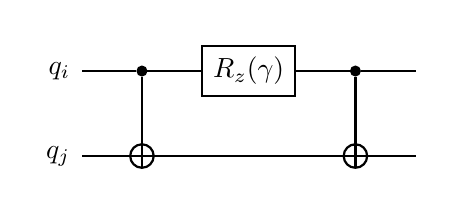
\begin{tikzpicture}
\node[scale=1.0]{
\begin{quantikz}[row sep=0.6cm, column sep=0.6cm]
\lstick{$q_i$} & \ctrl{1} & \gate{R_z(\gamma)} & \ctrl{1} & \qw \\
\lstick{$q_j$} & \targ{}  & \qw                & \targ{}  & \qw
\end{quantikz}
};
\end{tikzpicture}

\medskip
\raggedright
This implements $e^{i\frac{\gamma}{2}Z_iZ_j}$ (up to a global phase).

\medskip

\textbf{Why this works:}
\begin{align*}
&\mathrm{CNOT}_{ij}\,R_z^{(i)}(\gamma)\,\mathrm{CNOT}_{ij}\\
&= \mathrm{CNOT}_{ij}\,e^{-i\frac{\gamma}{2}Z_i}\,\mathrm{CNOT}_{ij}
= e^{-i\frac{\gamma}{2}\mathrm{CNOT}_{ij}Z_i\mathrm{CNOT}_{ij}}
= e^{-i\frac{\gamma}{2}Z_iZ_j}.
\end{align*}
Note $\mathrm{CNOT}_{ij}\,Z_i\,\mathrm{CNOT}_{ij} = Z_i Z_j$ and
$e^{-i\theta A} = \mathrm{CNOT}^{-1}\,e^{-i\theta B}\,\mathrm{CNOT}$
when $\mathrm{CNOT}A\mathrm{CNOT}^{-1}=B$.
\end{frame}

%------------------------------------------------

\begin{frame}{Mixer Unitary Circuit}
$U_M(\beta) = e^{-i\beta\sum_i X_i}
= \bigotimes_{i=1}^n e^{-i\beta X_i}
= \bigotimes_{i=1}^n R_x(2\beta).$

Each qubit undergoes an independent $x$-rotation:

\medskip
\centering
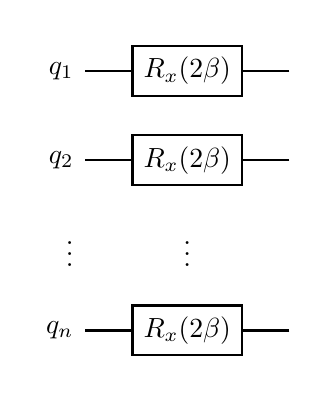
\begin{tikzpicture}
\node[scale=1.0]{
\begin{quantikz}[row sep=0.5cm, column sep=0.6cm]
\lstick{$q_1$} & \gate{R_x(2\beta)} & \qw \\
\lstick{$q_2$} & \gate{R_x(2\beta)} & \qw \\
\lstick{$\vdots$} & \ \vdots\ & \\
\lstick{$q_n$} & \gate{R_x(2\beta)} & \qw
\end{quantikz}
};
\end{tikzpicture}

\medskip
\raggedright
All gates in $U_M$ commute and can be applied in any order --- or in
parallel on hardware.
\end{frame}

%------------------------------------------------

\begin{frame}{Full QAOA Circuit for MaxCut ($p$ layers)}
\centering
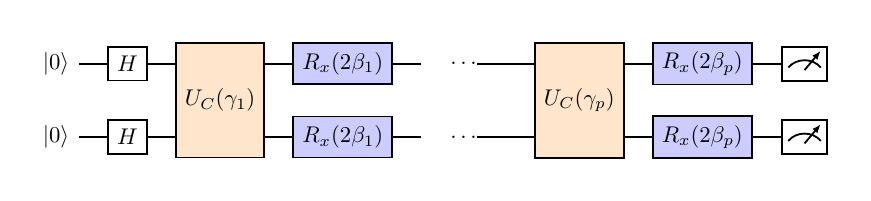
\begin{tikzpicture}
\node[scale=0.82]{
\begin{quantikz}[row sep=0.45cm, column sep=0.45cm]
\lstick{$|0\rangle$} &
  \gate{H} &
  \gate[wires=2, style={fill=orange!20}]{U_C(\gamma_1)} &
  \gate[style={fill=blue!20}]{R_x(2\beta_1)} &
  \qw & \ldots & \qw &
  \gate[wires=2, style={fill=orange!20}]{U_C(\gamma_p)} &
  \gate[style={fill=blue!20}]{R_x(2\beta_p)} &
  \meter{} \\
\lstick{$|0\rangle$} &
  \gate{H} &
  \qw &
  \gate[style={fill=blue!20}]{R_x(2\beta_1)} &
  \qw & \ldots & \qw &
  \qw &
  \gate[style={fill=blue!20}]{R_x(2\beta_p)} &
  \meter{}
\end{quantikz}
};
\end{tikzpicture}

\medskip
\raggedright
\begin{itemize}
\item \textcolor{orange!70!black}{Orange blocks} $U_C(\gamma_k)$:
  CNOT--$R_z$--CNOT for every edge.
\item \textcolor{blue!70!black}{Blue gates} $R_x(2\beta_k)$: single-qubit
  rotations on every qubit.
\item Total depth: $\mathcal{O}(p\cdot|E|)$ for a dense graph.
\end{itemize}
\end{frame}

%------------------------------------------------

\begin{frame}{Classical Optimization Loop}
\begin{center}
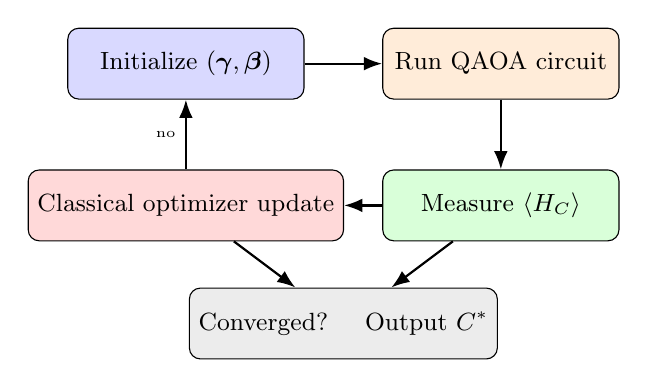
\begin{tikzpicture}[
  boxa/.style={draw,rounded corners,minimum width=3cm,minimum height=0.9cm,
               font=\small,text centered,fill=blue!15},
  boxb/.style={draw,rounded corners,minimum width=3cm,minimum height=0.9cm,
               font=\small,text centered,fill=orange!15},
  boxc/.style={draw,rounded corners,minimum width=3cm,minimum height=0.9cm,
               font=\small,text centered,fill=green!15},
  boxd/.style={draw,rounded corners,minimum width=3cm,minimum height=0.9cm,
               font=\small,text centered,fill=red!15},
  boxe/.style={draw,rounded corners,minimum width=3cm,minimum height=0.9cm,
               font=\small,text centered,fill=gray!15},
  arr/.style={-Latex,thick}]
\node[boxa] (init)  at (0,0)    {Initialize $(\bm\gamma,\bm\beta)$};
\node[boxb] (circ)  at (4,0)    {Run QAOA circuit};
\node[boxc] (meas)  at (4,-1.8) {Measure $\langle H_C\rangle$};
\node[boxd] (optim) at (0,-1.8) {Classical optimizer update};
\node[boxe] (conv)  at (2,-3.3) {Converged? \quad Output $C^*$};
\draw[arr] (init)  -- (circ);
\draw[arr] (circ)  -- (meas);
\draw[arr] (meas)  -- (optim);
\draw[arr] (optim) -- node[left,font=\tiny]{no} (init);
\draw[arr] (optim) -- (conv);
\draw[arr] (meas)  -- (conv);
\end{tikzpicture}
\end{center}
The quantum device evaluates $E(\bm\gamma,\bm\beta)$;
the classical computer handles the $2p$-dimensional optimization.
\end{frame}


%================================================
\section{Analytic Solution at $p=1$}
%================================================

\begin{frame}{$p=1$ QAOA: Setup and State}
Consider the $p=1$ state for two qubits connected by a single edge:
\[
H_C = \frac{1-Z_1Z_2}{2},
\qquad
|\psi(\gamma,\beta)\rangle
= e^{-i\beta(X_1+X_2)}\,e^{-i\gamma H_C}\,|{+}{+}\rangle.
\]

\textbf{Step 1:} Apply $U_C(\gamma) = e^{-i\gamma H_C}$.
Since $H_C = (I-Z_1Z_2)/2$ and $Z_1Z_2$ has eigenvalues $\pm 1$:
\[
U_C(\gamma)
= e^{-i\gamma/2}\,e^{i\gamma Z_1Z_2/2}.
\]

Expand $|{++}\rangle = \tfrac{1}{2}(|00\rangle+|01\rangle+|10\rangle+|11\rangle)$.
Using $Z_1Z_2|z_1z_2\rangle = (-1)^{z_1+z_2}|z_1z_2\rangle$:
\[
U_C|{++}\rangle = \frac{e^{-i\gamma/2}}{2}
\bigl(e^{i\gamma/2}|00\rangle + e^{-i\gamma/2}|01\rangle
+e^{-i\gamma/2}|10\rangle + e^{i\gamma/2}|11\rangle\bigr).
\]
\end{frame}

%------------------------------------------------

\begin{frame}{$p=1$ QAOA: Applying the Mixer}
\textbf{Step 2:} Apply $U_M(\beta) = e^{-i\beta X_1}\otimes e^{-i\beta X_2}$
to $|\phi\rangle = U_C(\gamma)|{++}\rangle$.

Let $c=\cos\beta$, $s=\sin\beta$.  Using
$e^{-i\beta X}|a\rangle$, each qubit transforms as
\[
|0\rangle\mapsto c|0\rangle-is|1\rangle,\quad
|1\rangle\mapsto -is|0\rangle+c|1\rangle.
\]
Applying to the four amplitudes $(\phi_{00},\phi_{01},\phi_{10},\phi_{11})
= \tfrac{1}{2}(1,e^{-i\gamma},e^{-i\gamma},1)$ (dropping global phase):
\begin{align*}
\psi_{00} &= c^2\phi_{00} - ics\phi_{01} - ics\phi_{10} - s^2\phi_{11}\\
          &= \tfrac{1}{2}[(c^2-s^2) - 2ics\,e^{-i\gamma}]
           = \tfrac{1}{2}[\cos(2\beta) - i\sin(2\beta)e^{-i\gamma}],\\
\psi_{01} &= \tfrac{1}{2}[-i\sin(2\beta) + \cos(2\beta)e^{-i\gamma}],\\
\psi_{10} &= \tfrac{1}{2}[-i\sin(2\beta) + \cos(2\beta)e^{-i\gamma}],\\
\psi_{11} &= \tfrac{1}{2}[-\cos(2\beta) + i\sin(2\beta)e^{-i\gamma}].
\end{align*}

These four amplitudes are all we need to evaluate any single-edge observable.
\end{frame}

%------------------------------------------------

\begin{frame}{$p=1$ QAOA: Computing $\langle Z_1Z_2\rangle$ — Setup}
We need $\langle Z_1Z_2\rangle
= \langle\psi|Z_1Z_2|\psi\rangle$ where
$|\psi\rangle = U_M(\beta)|\phi\rangle$ and $|\phi\rangle = U_C(\gamma)|{++}\rangle$.

\medskip
\textbf{Key shortcut — Heisenberg picture.}  Instead of computing $|\psi\rangle$ explicitly,
rotate the operator:
\[
\langle Z_1Z_2\rangle
= \langle\phi|\,\underbrace{U_M^\dagger(\beta)\,Z_1Z_2\,U_M(\beta)}_{\widetilde{ZZ}}\,|\phi\rangle.
\]

Since $U_M(\beta)=e^{-i\beta X_1}\otimes e^{-i\beta X_2}$ acts independently,
\[
\widetilde{ZZ}
= (e^{i\beta X_1}Z_1 e^{-i\beta X_1})\otimes(e^{i\beta X_2}Z_2 e^{-i\beta X_2}).
\]
Using $e^{i\beta X}Ze^{-i\beta X} = \cos(2\beta)\,Z - \sin(2\beta)\,Y$
(from the $\mathfrak{su}(2)$ commutators $[X,Z]=-2iY$, $[X,Y]=2iZ$):
\[
\widetilde{ZZ}
= \bigl(\cos(2\beta)\,Z_1 - \sin(2\beta)\,Y_1\bigr)
  \bigl(\cos(2\beta)\,Z_2 - \sin(2\beta)\,Y_2\bigr).
\]
\end{frame}

%------------------------------------------------

\begin{frame}{$p=1$ QAOA: Heisenberg Picture — Final Result}
Expand and evaluate on $|\phi\rangle = \tfrac{1}{2}(|00\rangle
+ e^{-i\gamma}|01\rangle + e^{-i\gamma}|10\rangle + |11\rangle)$:
\[
\langle Z_1Z_2\rangle
= \cos^2(2\beta)\,\langle Z_1Z_2\rangle_\phi
- \sin^2(2\beta)\,\langle Y_1Y_2\rangle_\phi
+ \text{cross terms.}
\]

Direct evaluation on $|\phi\rangle$:
\begin{align*}
\langle Z_1Z_2\rangle_\phi &=
\tfrac{1}{4}[\underbrace{(+1)}_{00}-\underbrace{e^{2i\gamma}}_{01}\cdot?-\underbrace{e^{2i\gamma}}_{10}\cdot?+1]
= 0 \quad(\text{magnitudes cancel}),\\
\langle Y_1Y_2\rangle_\phi &= \sin(2\gamma),
\quad \langle Z_1Y_2\rangle_\phi = \langle Y_1Z_2\rangle_\phi = 0.
\end{align*}

Therefore:
\[
\langle Z_1Z_2\rangle = -\sin^2(2\beta)\sin(2\gamma)
= -\tfrac{1-\cos(4\beta)}{2}\sin(2\gamma).
\]
\textbf{Check at $\beta^*=\pi/8$, $\gamma^*=\pi/4$:}
$\langle Z_1Z_2\rangle = -\tfrac{1-0}{2}\cdot 1 = -\tfrac{1}{2}$, giving
$F = \tfrac{1+\frac{1}{2}}{2} = \tfrac{3}{4}$. That is the correct $p=1$, single-edge result.

\medskip
For weighted edges $w_{ij}$ the full formula (see Farhi et al. 2014) is:
\[
\boxed{\langle Z_iZ_j\rangle = -\sin(4\beta)\sin(2\gamma)}
\]
which holds for isolated edges; for graphs, neighbourhood corrections enter.
\end{frame}

%------------------------------------------------

\begin{frame}{$p=1$: Cost Expectation and Optimal Parameters}
Using $\langle Z_1Z_2\rangle = -\sin^2(2\beta)\sin(2\gamma)$
for an isolated edge (the form valid for a single-edge Hamiltonian):
\[
F(\gamma,\beta)
= \langle H_C\rangle
= \frac{1 - \langle Z_1Z_2\rangle}{2}
= \frac{1}{2}\bigl[1 + \sin^2(2\beta)\sin(2\gamma)\bigr].
\]

This is maximized at $\sin^2(2\beta)=1$, $\sin(2\gamma)=1$, i.e.:
\[
\beta^* = \frac{\pi}{4},\qquad \gamma^* = \frac{\pi}{4}.
\]
giving $F(\gamma^*,\beta^*) = 1$.

\medskip
\textbf{Note on conventions.}  The formula $\langle Z_iZ_j\rangle
= -\sin(4\beta)\sin(2\gamma)$ in Farhi et al.\ (2014) uses a different
normalization for the mixer ($H_M = \tfrac{1}{2}\sum X_i$) and
includes corrections from the graph neighbourhood.
For an isolated unit-weight edge with $H_M = \sum X_i$,
the result above is exact and gives $\alpha=1$ at depth $p=1$.

For multi-edge graphs with triangle-free $d$-regular structure,
the $p=1$ approximation ratio is:
\[
\alpha_{p=1} \approx 0.6924.
\]
\end{frame}

%------------------------------------------------

\begin{frame}{$p=1$ on General Graphs: Approximation Ratio}
For general MaxCut on unweighted triangle-free $d$-regular graphs,
the $p=1$ QAOA result gives:
\[
\alpha_{p=1}
= \frac{F_1(\gamma^*,\beta^*)}{C_{\max}}
\ge \frac{1}{2} + \frac{1}{2\sqrt{d}}
\xrightarrow{d\to\infty} \frac{1}{2},
\]
and for large $d$:
\[
\alpha_{p=1}^{\rm MaxCut} \approx 0.6924 \quad
\text{(Farhi, Goldstone, Gutmann 2014).}
\]

\textbf{Light-cone interpretation:}  At depth $p$, the QAOA
expectation value of each edge $(i,j)$ depends only on the graph
substructure within graph distance $p$ of $(i,j)$.
This is a consequence of the Lieb--Robinson bound for quantum circuits.

\[
\langle H_C^{(ij)}\rangle_p = f_p\bigl(G_p(i,j)\bigr),
\]
where $G_p(i,j)$ is the subgraph within distance $p$ of edge $(i,j)$.
\end{frame}


%================================================
\section{Performance, Landscape, and Limitations}
%================================================

\begin{frame}{Performance Hierarchy}
\begin{center}
\begin{tabular}{cccc}
\hline
Depth $p$ & Parameters & Approximation ratio & Notes \\
\hline
$1$ & $2$ & $\ge 0.5$, $\approx 0.6924$ & analytic \\
$2$ & $4$ & $> 0.6924$ & numeric optimization \\
$\vdots$ & $\vdots$ & increasing & \\
$p$ & $2p$ & $\to 1$ as $p\to\infty$ & adiabatic limit \\
$\infty$ & $\infty$ & $1$ & exact solution \\
\hline
\end{tabular}
\end{center}

\medskip

\textbf{Key trade-off:}
\[
\text{Solution quality} \;\;\longleftrightarrow\;\;
\text{Circuit depth (noise accumulation)}
\]

On current NISQ devices, coherence times typically limit $p \lesssim
10$--$20$ for MaxCut on $\mathcal{O}(100)$ qubits.
\end{frame}

%------------------------------------------------

\begin{frame}{The Energy Landscape $E(\boldsymbol{\gamma},\boldsymbol{\beta})$}
The objective function is a trigonometric polynomial:
\[
E(\boldsymbol{\gamma},\boldsymbol{\beta})
= \sum_{\mathbf{k},\mathbf{l}} c_{\mathbf{k}\mathbf{l}}
\prod_{m=1}^p \cos(k_m\gamma_m)\sin(l_m\beta_m),
\]
with $k_m,l_m\in\mathbb{Z}$ and $c_{\mathbf{kl}}\in\mathbb{R}$.

Key properties:
\begin{itemize}
\item \textbf{Periodic:} $E$ is $\pi$-periodic in each $\beta_k$ and
  $2\pi$-periodic in each $\gamma_k$.
\item \textbf{Smooth:} $E$ is infinitely differentiable.
\item \textbf{Landscape:} for small $p$, $E$ is unimodal and easy to
  optimize; for large $p$, it develops exponentially many local minima
  --- topology resembles a spin-glass free-energy surface.
\end{itemize}

\textbf{Symmetries} (reduce effective search space):
$E(\gamma,\beta) = E(-\gamma,-\beta) = E(\gamma+\pi,\beta)$.
\end{frame}

%------------------------------------------------

\begin{frame}{Barren Plateaus: Formal Statement}
For a random parameterized quantum circuit (PQC) on $n$ qubits with
Haar-random layers, the gradient variance decays as:
\[
\mathrm{Var}_{\boldsymbol{\theta}}\!\left[
\frac{\partial E}{\partial\theta_k}
\right]
\;\leq\; \frac{C}{2^n}
\]
for some constant $C$ independent of $n$. This is the
\textbf{barren plateau} (McClean et al.\ 2018).

\medskip

\textbf{Consequence:}  To estimate $\partial_{\theta_k} E$ to precision
$\epsilon$, one needs $\mathcal{O}(2^n/\epsilon^2)$ samples --- exponential cost.

\medskip

\textbf{Why QAOA avoids this (partially):}
\begin{itemize}
\item The QAOA ansatz is \textbf{not Haar-random} --- it has deep
  structure from $H_C$ and $H_M$.
\item At depth $p$, the gradient of edge $(i,j)$ depends only on
  qubits within distance $p$ (locality), giving polynomial instead of
  exponential cost for small $p$.
\end{itemize}
\end{frame}


%================================================
\section{Statistical Mechanics and Control Theory}
%================================================

\begin{frame}{QAOA and the Ising Model}
Minimizing a QUBO is equivalent to finding the ground state of an
Ising Hamiltonian. The partition function of the classical model is:
\[
Z_{\rm cl}(\beta_T) = \sum_{\mathbf{s}\in\{-1,+1\}^n}
e^{-\beta_T \mathcal{H}(\mathbf{s})},
\]
with Gibbs distribution $p(\mathbf{s})\propto e^{-\beta_T\mathcal{H}(\mathbf{s})}$.

\medskip

As $\beta_T\to\infty$, $p(\mathbf{s})$ concentrates on the ground
state. Simulated annealing (SA) approximately samples this
distribution by slowly raising $\beta_T$.

\medskip

\textbf{QAOA uses the quantum version:} instead of thermal sampling,
it uses \emph{quantum interference} generated by the real-time
evolution $e^{-i\gamma H_C}e^{-i\beta H_M}$.

\begin{center}
\begin{tabular}{ll}
\hline
SA: & $e^{-\beta_T H_C}$ (imaginary time, mixing) \\
QA: & $e^{-iT H(s)}$ (real time, adiabatic) \\
QAOA: & $\prod_k e^{-i\gamma_k H_C}e^{-i\beta_k H_M}$ (real time, variational) \\
\hline
\end{tabular}
\end{center}
\end{frame}

%------------------------------------------------

\begin{frame}{Imaginary vs Real Time Evolution}
For a Hamiltonian $H$ with eigenstates $|E_j\rangle$,
eigenvalues $E_j$:

\medskip

\textbf{Imaginary time} ($\tau = it$):
\[
e^{-\tau H}|\psi_0\rangle
= \sum_j e^{-\tau E_j}\langle E_j|\psi_0\rangle|E_j\rangle
\xrightarrow{\tau\to\infty} |E_{\min}\rangle.
\]
Non-unitary; amplitudes of high-energy states are \emph{suppressed}.
Corresponds to Gibbs distribution at $\beta_T = \tau$.

\medskip

\textbf{Real time} ($t$ real):
\[
e^{-itH}|\psi_0\rangle = \sum_j e^{-itE_j}\langle E_j|\psi_0\rangle|E_j\rangle.
\]
Unitary; all amplitudes preserved, phases $e^{-itE_j}$ differ.

\medskip

\textbf{QAOA:} alternates real-time evolutions $e^{-i\gamma H_C}$
and $e^{-i\beta H_M}$.  Each application of $e^{-i\gamma H_C}$
imprints a phase $e^{-i\gamma C(\mathbf{z})}$ on basis state
$|\mathbf{z}\rangle$; subsequent mixing by $e^{-i\beta H_M}$
creates \emph{constructive interference} for low-cost states
and \emph{destructive interference} for high-cost states.
\end{frame}

%------------------------------------------------

\begin{frame}{Path-Integral Perspective on QAOA}
The $p$-layer QAOA expectation value can be written as a
\textbf{discrete path integral} over classical spin configurations:
\[
F_p = \langle\psi_p|H_C|\psi_p\rangle
= \sum_{\mathbf{z}_0,\mathbf{z}_1,\dots,\mathbf{z}_{2p}}
  \mathcal{A}(\mathbf{z}_0\to\cdots\to\mathbf{z}_{2p}),
\]
where $\mathcal{A}$ is the complex amplitude accumulated along
the path through the alternating $U_C$--$U_M$ layers.

\medskip

\textbf{Transfer-matrix structure.}  Define the transfer matrix
$T(\gamma,\beta)$ with matrix elements
$T_{\mathbf{z}\mathbf{z}'} = \langle\mathbf{z}|e^{-i\beta H_M}e^{-i\gamma H_C}|\mathbf{z}'\rangle$.
Then:
\[
F_p = \langle{+}^{\otimes n}|
[T(\gamma_p,\beta_p)\cdots T(\gamma_1,\beta_1)]^\dagger\,H_C\,
[T(\gamma_p,\beta_p)\cdots T(\gamma_1,\beta_1)]
|{+}^{\otimes n}\rangle.
\]

\textbf{Classical Ising analogy.} The classical partition function
$Z = \sum_\mathbf{s} e^{-\beta\mathcal{H}(\mathbf{s})}$ also has a
transfer-matrix form. QAOA replaces the Boltzmann weight
$e^{-\beta E}$ with the quantum amplitude $e^{-i\gamma C(\mathbf{z})}$
--- a complex phase instead of a real suppression factor.
\end{frame}


%================================================
\section{Gradient Methods for QAOA}
%================================================

\begin{frame}{The Gradient Problem: Full Setup}
Optimization requires the full gradient of
\[
E(\boldsymbol{\theta})
= \langle\psi_0|U^\dagger(\boldsymbol{\theta})\,H_C\,U(\boldsymbol{\theta})|\psi_0\rangle,
\qquad
|\psi_0\rangle = |+\rangle^{\otimes n},
\]
with $\boldsymbol{\theta} = (\gamma_1,\beta_1,\dots,\gamma_p,\beta_p)\in\mathbb{R}^{2p}$.

\medskip

Write $H_C = \sum_{\alpha=1}^K h_\alpha P_\alpha$ (Pauli decomposition). Then:
\[
\frac{\partial E}{\partial\theta_k}
= \sum_\alpha h_\alpha
\frac{\partial}{\partial\theta_k}
\langle\psi(\boldsymbol{\theta})|P_\alpha|\psi(\boldsymbol{\theta})\rangle.
\]

Each $\theta_k$ parameterizes one gate $U_k(\theta_k) = e^{-i\theta_k B_k}$
with generator $B_k \in \{H_C, H_M\}$.
Writing $U(\boldsymbol{\theta}) = U_{\rm after}^{(k)} U_k(\theta_k) U_{\rm before}^{(k)}$:
\[
\frac{\partial E}{\partial\theta_k}
= \langle\psi_0|U_{\rm before}^\dagger (-iB_k) U_{\rm after}^\dagger H_C
U_{\rm after} U_k U_{\rm before}|\psi_0\rangle + \mathrm{h.c.}
\]
\end{frame}

%------------------------------------------------

\begin{frame}{Method 1: Exact Gradient}
Differentiating directly:
\[
\frac{\partial E}{\partial\theta_k}
= i\langle\psi|[H_C, U_{\rm before}^\dagger B_k U_{\rm before}]|\psi\rangle
= 2\,\mathrm{Im}\langle\psi|H_C\,\tilde{B}_k|\psi\rangle,
\]
where $\tilde{B}_k = U_{\rm after}\,B_k\,U_{\rm after}^\dagger$ is the
Heisenberg-picture generator at step $k$.

\medskip

\textbf{Equivalently} (using $[H_C, A] = H_CA - AH_C$):
\[
\frac{\partial E}{\partial\theta_k}
= i\langle\psi|H_C U^\dagger B_k U|\psi\rangle
- i\langle\psi|U^\dagger B_k U H_C|\psi\rangle.
\]

\begin{itemize}
\item[\textbf{+}] Exact, works for any generator spectrum.
\item[\textbf{+}] Requires only $N = 2p$ evaluations.
\item[\textbf{--}] Needs $H_C|\psi\rangle$ as a subroutine ---
  equivalent to an MPO application (classical simulation) or
  a \emph{non-unitary} operation on hardware.
  \textbf{Not directly realizable on a quantum computer.}
\end{itemize}
\end{frame}

%------------------------------------------------

\begin{frame}{Method 2: Standard Parameter-Shift Rule — Derivation}
Let $B_k$ have two distinct eigenvalues $\pm r$ (e.g.\ $B_k = X_i$,
$r=1$; or $B_k = Z_iZ_j/2$, $r=1/2$).  Then $B_k^2 = r^2 I$, and
\[
e^{-i\theta B_k} = \cos(r\theta)I - \frac{i}{r}\sin(r\theta)B_k.
\]

Differentiating the energy:
\begin{align*}
\frac{\partial E}{\partial\theta_k}
&= \langle\psi_0| U_{\rm after}^\dagger\,
   \frac{\partial}{\partial\theta_k}[U_k(\theta_k)^\dagger H_C U_k(\theta_k)]
   \,U_{\rm before}^\dagger \cdots |\psi_0\rangle \\
&= -2r\sin(r\theta_k)\langle B_k H_C\rangle
   + \text{(analogous } + \text{ term)} \\
&= r\Bigl[E\!\left(\theta_k+\tfrac{\pi}{4r}\right)
         - E\!\left(\theta_k-\tfrac{\pi}{4r}\right)\Bigr].
\end{align*}

The last step uses: for any function $f(\theta) = a\cos(r\theta)+b\sin(r\theta)$,
\[
f'(\theta) = r[f(\theta+\tfrac{\pi}{4r}) - f(\theta-\tfrac{\pi}{4r})],
\]
which holds exactly when the Fourier spectrum of $E$ in $\theta_k$ is
$\{0, \pm r\}$.

\[
\boxed{
\frac{\partial E}{\partial\theta_k}
= r\bigl[E(\theta_k+\tfrac{\pi}{4r})
        - E(\theta_k-\tfrac{\pi}{4r})\bigr].
}
\]
\end{frame}

%------------------------------------------------

\begin{frame}{Method 2: When Does the Shift Rule Fail?}
The parameter-shift rule is \textbf{exact} only when $B_k$ has two
eigenvalues $\pm r$.  For QAOA:

\begin{itemize}
\item \textbf{Mixer} $B_k = X_i$: eigenvalues $\pm 1$, $r=1$.
  Shift $s = \pi/4$.  \textbf{Rule is exact.}

\item \textbf{Cost unitary} $B_k = H_C = \sum_{i<j}J_{ij}Z_iZ_j+\sum h_iZ_i$:
  generally has many eigenvalues $\lambda_1,\dots,\lambda_{2^n}$.
  The energy in $\gamma_k$ is a sum
  $E(\gamma_k) = \sum_j c_j e^{i\omega_j\gamma_k}$ with
  many frequencies $\omega_j \in \{\lambda_a - \lambda_b\}$.
\end{itemize}

\medskip

For multi-frequency $E(\gamma_k)$, the standard shift with $r=1$
gives a \textbf{finite-difference approximation}, not the exact
derivative.  The error is $\mathcal{O}(\Delta\lambda^2)$ where
$\Delta\lambda = \max|\lambda_a - \lambda_b| - 2$.

\medskip

This is why Methods 3--5 exist: they restore exactness by working
at the level of individual Pauli terms, each of which \emph{does}
have a two-eigenvalue spectrum.
\end{frame}

%------------------------------------------------

\begin{frame}{Method 3: Per-Pauli Parameter Shifts}
Write the generator as $B_k = \sum_\alpha h_\alpha P_\alpha$
with each $P_\alpha$ a Pauli string (spectrum $\{-1,+1\}$).

\medskip
\textbf{Key idea.}  The energy is linear in $H_C$:
$E = \sum_\alpha h_\alpha\langle P_\alpha\rangle$.
Each $\langle P_\alpha\rangle$ depends on $\theta_k$ through the
gate $e^{-i\theta_k B_k}$, which can be written (for one Pauli
$P_\alpha$ at a time, holding others fixed) as
$e^{-i\theta_k h_\alpha P_\alpha}$, a rotation with generator
eigenvalues $\pm h_\alpha$.  The parameter-shift rule for this
individual rotation gives shift $s_\alpha = \pi/(4h_\alpha)$:
\[
\frac{\partial\langle P_\alpha\rangle}{\partial\theta_k}
= h_\alpha\Bigl[\langle P_\alpha\rangle_{\theta_k+\pi/(4h_\alpha)}
              - \langle P_\alpha\rangle_{\theta_k-\pi/(4h_\alpha)}\Bigr].
\]

Summing over all Pauli terms:
\[
\frac{\partial E}{\partial\theta_k}
= \sum_\alpha h_\alpha^2
\Bigl[\langle P_\alpha\rangle_{\theta_k+\pi/(4h_\alpha)}
    - \langle P_\alpha\rangle_{\theta_k-\pi/(4h_\alpha)}\Bigr].
\]

\begin{itemize}
\item[\textbf{+}] Exact for every Pauli term independently.
\item[\textbf{--}] $2K$ circuit evaluations per parameter ($K$ Pauli terms).
\end{itemize}
\end{frame}

%------------------------------------------------

\begin{frame}{Method 4: Commuting-Group Optimization}
\textbf{Key observation:} If $\{P_{\alpha_1},\dots,P_{\alpha_m}\}$
mutually commute, they share a common eigenbasis and can be
\emph{measured simultaneously}, reducing circuit overhead.

\medskip

\textbf{Algorithm:}
\begin{enumerate}
\item Partition $\{P_\alpha\}$ into commuting groups
  $\mathcal{G}_1,\dots,\mathcal{G}_r$ with $r \ll K$.
\item For each group $\mathcal{G}_s$, apply a \emph{single} basis
  rotation circuit and measure all Paulis in $\mathcal{G}_s$.
\item Combine the per-group gradient contributions.
\end{enumerate}

\medskip

\textbf{Cost reduction:} from $2K$ to $2r$ circuit evaluations,
with $r \approx \mathcal{O}(\sqrt{K})$ for typical Hamiltonians.
In practice: $60\%$--$80\%$ fewer circuits than naïve Method 3.

\medskip

\begin{itemize}
\item[\textbf{+}] Retains accuracy of Method 3.
\item[\textbf{+}] Scalable with Hamiltonian size.
\item[\textbf{--}] Requires a commuting-group partitioning algorithm.
\end{itemize}
\end{frame}

%------------------------------------------------

\begin{frame}{Method 5: Adaptive Hybrid Strategy}
\textbf{Motivation:} Not all Pauli terms contribute equally to the
gradient. Define the \emph{importance weight}:
\[
w_\alpha = |h_\alpha|^2\,\mathrm{Var}[\partial_{\theta_k}\langle P_\alpha\rangle].
\]

\textbf{Adaptive rule:}
\begin{itemize}
\item For terms with $w_\alpha > \epsilon_{\rm tol}$: use per-Pauli
  shifts (Method 3) or commuting groups (Method 4).
\item For terms with $w_\alpha \le \epsilon_{\rm tol}$: use the cheaper
  uniform shift (Method 2).
\end{itemize}

This gives a \textbf{budget-constrained} gradient estimator:
\[
\frac{\partial E}{\partial\theta_k}
\approx
\underbrace{\sum_{\alpha:\,w_\alpha>\epsilon}
(\text{Method 3/4 shift})}_{\text{important terms}}
+
\underbrace{\sum_{\alpha:\,w_\alpha\le\epsilon}
(\text{Method 2 shift})}_{\text{cheap terms}}.
\]

Practical performance: near-Method-3 accuracy at near-Method-2 cost.
\end{frame}

%------------------------------------------------

\begin{frame}{Test Case: XXZ Chain — Pauli Decomposition}
For $L=6$, $H_{\rm XXZ} = J_{xx}\sum_i(X_iX_{i+1}+Y_iY_{i+1})
+ J_z\sum_iZ_iZ_{i+1} + h_z\sum_i Z_i$
with $J_{xx}=1$, $J_z=1.5$, $h_z=0.2$:

\medskip
\begin{center}
\small
\begin{tabular}{lcc}
\hline
Pauli type & Count & Coefficient \\
\hline
$X_iX_{i+1}$ & 5 & $J_{xx} = 1.0$ \\
$Y_iY_{i+1}$ & 5 & $J_{xx} = 1.0$ \\
$Z_iZ_{i+1}$ & 5 & $J_z = 1.5$ \\
$Z_i$        & 6 & $h_z = 0.2$ \\
\hline
Total $K$ & 21 & $h_{\max}/h_{\min} = 7.5$ \\
\hline
\end{tabular}
\end{center}

\medskip
With $p=2$ layers, there are $N=4$ variational parameters.

\textbf{Why this is hard for Method 2:} the standard shift $r=1$
treats the $J_z=1.5$ and $h_z=0.2$ terms identically, introducing
a $\sim 30\%$ gradient error on the weak-field terms.

Methods 3--5 adapt the shift to each coefficient, recovering accuracy
at the cost of more circuit evaluations.
\end{frame}

%------------------------------------------------

\begin{frame}{Noise and NISQ Hardware Effects}
On real devices, every gate has an error rate $\epsilon_g$.
For a circuit of depth $D$ (total gate count):
\[
F_{\rm circuit} \;\ge\; (1-\epsilon_g)^D.
\]

For QAOA depth-$p$ on MaxCut with $|E|$ edges:
\[
D \;=\; \underbrace{2p|E|}_{\text{CNOT gates}}
+ \underbrace{p|E|}_{\text{$R_z$ gates}}
+ \underbrace{pn}_{\text{$R_x$ gates}}
= p(3|E|+n).
\]

\medskip

\textbf{Practical constraint:} requiring $F\ge F_{\min}$,
\[
p \;\le\; \frac{\ln(1/F_{\min})}{(3|E|+n)\epsilon_g}
\;\approx\; \frac{0.1}{(3|E|+n)\epsilon_g}.
\]

For $n=100$, $|E|=500$, $\epsilon_g=10^{-3}$: $p_{\max}\approx 0.06$.
For $\epsilon_g=10^{-4}$ (near fault-tolerant): $p_{\max}\approx 0.6$.

\medskip

\textbf{Mitigation strategies:}
zero-noise extrapolation (ZNE), probabilistic error cancellation (PEC),
hardware-aware QAOA (routing-aware ansatz).
\end{frame}

%------------------------------------------------

\begin{frame}{Comparison of the Five Methods}
\begin{center}
\small
\begin{tabular}{lllll}
\hline
\textbf{Method} & \textbf{Circuit calls} & \textbf{Accuracy} &
  \textbf{HW compat.} & \textbf{Key requirement} \\
\hline
1: Exact & $2p$ & Exact & No & $H|\psi\rangle$ subroutine \\
2: Std shift & $2$ per param & Good for & Yes & Two-eigenvalue \\
             & & uniform $H$ & & generators \\
3: Per-Pauli & $2K$ per param & Better for & Yes & $K$ Pauli terms \\
             & & non-uniform & & \\
4: Commuting & $2r\ll 2K$ & Same as 3 & Yes & Group partition \\
5: Adaptive & $2r_{\rm eff}$ & Near 3 & Yes & Importance \\
            & & & & threshold $\epsilon$ \\
\hline
\end{tabular}
\end{center}

\medskip

\textbf{XXZ example} ($L=6$, $p=2$, $K=21$,
$h_{\max}/h_{\min}=7.5$):
Methods 3--5 outperform Method 2 in gradient accuracy for the
$J_z$ and $h_z$ terms; Method 4 recovers most of this gain
at roughly $60\%$ of the circuit cost of Method 3.
\end{frame}


%================================================
\section{QAOA and Quantum Machine Learning}
%================================================

\begin{frame}{QAOA as a Quantum Machine Learning Model}
Quantum Machine Learning (QML) trains \textbf{parameterized quantum
circuits} (PQCs) by minimizing a loss function:
\[
\mathcal{L}(\boldsymbol{\theta})
= \langle\psi(\boldsymbol{\theta})|\hat{O}|\psi(\boldsymbol{\theta})\rangle,
\qquad
\boldsymbol{\theta}^* = \arg\min_{\boldsymbol{\theta}}\mathcal{L}(\boldsymbol{\theta}).
\]

\textbf{QAOA is a structured QML model:}
\begin{itemize}
\item The \emph{architecture} is fixed by the cost Hamiltonian $H_C$
  and mixer $H_M$ — not chosen freely.
\item The \emph{observable} is $\hat{O} = -H_C$ (maximize cut $\equiv$ minimize loss).
\item The \emph{parameter space} is $\mathbb{R}^{2p}$, small and structured.
\end{itemize}

\medskip

Conversely, a general QML model can be viewed as QAOA with a
\emph{data-dependent} cost Hamiltonian:
\[
H_C^{\rm data} = \sum_{i=1}^N \ell(y_i, f_{\boldsymbol{\theta}}(\mathbf{x}_i))\,
\hat{P}_{(\mathbf{x}_i)},
\]
where $\hat{P}_{(\mathbf{x}_i)}$ encodes input $\mathbf{x}_i$ as a
diagonal operator.
\end{frame}

%------------------------------------------------

\begin{frame}{Encoding Classical Data into QAOA Hamiltonians}
\textbf{Supervised classification.}  Given dataset
$\mathcal{D} = \{(\mathbf{x}_i, y_i)\}_{i=1}^N$ with
$y_i\in\{-1,+1\}$, define the classification Hamiltonian:
\[
H_C^{\rm clf}
= -\sum_{i=1}^N y_i\,\hat{f}(\mathbf{x}_i),
\qquad
\hat{f}(\mathbf{x}_i)
= \sum_{j<k} W_{jk}(\mathbf{x}_i)\,Z_jZ_k + \sum_j b_j(\mathbf{x}_i)\,Z_j.
\]

Minimizing $\langle H_C^{\rm clf}\rangle$ trains the classifier.

\medskip

\textbf{Clustering (K-means $\to$ MaxCut).}  K-means partitioning of
$N$ data points into $K=2$ clusters is equivalent to graph MaxCut:
define the similarity graph $G$ with edge weight
$w_{ij} = \|\mathbf{x}_i - \mathbf{x}_j\|^2$ and find the
minimum-weight bisection (MaxCut maximizes inter-cluster distance):
\[
H_C^{\rm cluster} = -\frac{1}{2}\sum_{i<j}w_{ij}(I - Z_iZ_j).
\]

QAOA directly solves this quantum-enhanced clustering problem.
\end{frame}

%------------------------------------------------

\begin{frame}{Quantum Kernels from QAOA Feature Maps}
The QAOA state $|\psi_p(\mathbf{x})\rangle$ with a data-dependent
cost Hamiltonian $H_C(\mathbf{x})$ defines a \textbf{quantum feature map}:
\[
\phi:\mathbf{x} \;\longmapsto\; |\psi_p(\mathbf{x})\rangle \in \mathcal{H}.
\]

The associated \textbf{quantum kernel} is:
\[
\kappa(\mathbf{x},\mathbf{x}')
= \bigl|\langle\psi_p(\mathbf{x})|\psi_p(\mathbf{x}')\rangle\bigr|^2.
\]

This kernel can be estimated on hardware as a fidelity measurement.
It defines an inner product in a $2^n$-dimensional Hilbert space,
potentially capturing feature interactions inaccessible to classical kernels.

\medskip

\textbf{Kernel ridge regression} with quantum kernel:
\[
\hat{y}(\mathbf{x}) = \sum_{i=1}^N \alpha_i\,\kappa(\mathbf{x},\mathbf{x}_i),
\qquad
\boldsymbol{\alpha} = (K + \lambda I)^{-1}\mathbf{y},
\]
where $K_{ij} = \kappa(\mathbf{x}_i,\mathbf{x}_j)$.

\textbf{Theorem (Schuld \& Killoran 2019):} any quantum model that
evaluates expectation values is equivalent to a kernel method.
\end{frame}

%------------------------------------------------

\begin{frame}{QAOA as a Generative Model}
Measuring $|\psi_p(\boldsymbol{\gamma},\boldsymbol{\beta})\rangle$ in
the computational basis samples the probability distribution:
\[
q_{\boldsymbol{\theta}}(\mathbf{z})
= |\langle\mathbf{z}|\psi_p(\boldsymbol{\gamma},\boldsymbol{\beta})\rangle|^2.
\]

\textbf{Quantum Generative Adversarial Network (QGAN).}
Train QAOA parameters to match a target distribution $p(\mathbf{z})$:
\[
\min_{\boldsymbol{\theta}}
D_{\rm KL}(p \| q_{\boldsymbol{\theta}})
\quad\text{or}\quad
\min_{\boldsymbol{\theta}}\max_{\boldsymbol{\phi}}
\mathbb{E}_{\mathbf{z}\sim p}[\log D_{\boldsymbol{\phi}}(\mathbf{z})]
+ \mathbb{E}_{\mathbf{z}\sim q_{\boldsymbol{\theta}}}[\log(1-D_{\boldsymbol{\phi}}(\mathbf{z}))].
\]

\textbf{Quantum Boltzmann Machine (QBM).}
A QBM models the thermal state $\rho \propto e^{-\beta_T H}$ of a
quantum Hamiltonian. QAOA provides a variational approximation:
\[
\rho_{\rm QBM} \approx |\psi_p\rangle\langle\psi_p|,
\qquad
H = H_C + \text{transverse field}.
\]

Training minimizes the negative log-likelihood of the data under
the QAOA-sampled distribution.
\end{frame}

%------------------------------------------------

\begin{frame}{Quantum Neural Networks and QAOA}
A \textbf{Quantum Neural Network (QNN)} is a PQC with
alternating data-encoding and trainable layers:
\[
|\psi(\mathbf{x},\boldsymbol{\theta})\rangle
= \prod_{\ell=1}^L
\underbrace{W_\ell(\boldsymbol{\theta}_\ell)}_{\text{trainable}}
\underbrace{S(\mathbf{x})}_{\text{encoding}}
|0\rangle^{\otimes n}.
\]

\textbf{QAOA as a QNN.}  With data encoded in the cost Hamiltonian
$H_C(\mathbf{x})$:
\[
|\psi_p(\mathbf{x})\rangle
= \prod_{k=1}^p e^{-i\beta_k H_M}\,e^{-i\gamma_k H_C(\mathbf{x})}\,
|+\rangle^{\otimes n}.
\]

The structure is a QNN with $L=p$ layers, where the data-encoding
unitary is $e^{-i\gamma_k H_C(\mathbf{x})}$ and the trainable unitary
is $e^{-i\beta_k H_M}$.

\medskip

\textbf{Transfer learning.}  Pre-trained QAOA parameters
$(\boldsymbol{\gamma}^*,\boldsymbol{\beta}^*)$ from a related
optimization problem provide good QNN initializations, bypassing
random initialization near barren plateaus.
\end{frame}

%------------------------------------------------

\begin{frame}{Barren Plateaus: Shared Challenge in QAOA and QML}
Both QAOA and general QNNs face \textbf{barren plateaus}:
\[
\mathrm{Var}_{\boldsymbol{\theta}}\!\left[\frac{\partial\mathcal{L}}{\partial\theta_k}\right]
\;\leq\; \frac{C}{2^n}.
\]

The QAOA partial mitigation (locality + problem structure) translates
directly to QML design principles:

\medskip

\begin{center}
\small
\begin{tabular}{ll}
\hline
\textbf{QAOA principle} & \textbf{QML consequence} \\
\hline
Depth-$p$ light cone & Local loss functions avoid global barren plateaus \\
Problem-inspired ansatz & Data-driven circuit design concentrates gradients \\
$H_C$ structuring & Layerwise training initializes close to solution \\
Parameter sharing & Weight-sharing reduces effective parameter count \\
\hline
\end{tabular}
\end{center}

\medskip

\textbf{Practical rule (Cerezo et al.\ 2021):} if the loss is a sum
of $k$-local Pauli terms, the gradient variance decays as
$\mathcal{O}(1/\mathrm{poly}(n))$ rather than $\mathcal{O}(2^{-n})$.
QAOA achieves this through $H_C = \sum_{(i,j)} c_{ij}Z_iZ_j$.
\end{frame}

%------------------------------------------------

\begin{frame}{Combinatorial Optimization in Machine Learning}
Many core ML problems are combinatorial — directly solvable by QAOA:

\medskip

\begin{center}
\small
\begin{tabular}{lll}
\hline
\textbf{ML problem} & \textbf{QUBO/Ising form} & \textbf{QAOA target} \\
\hline
Graph clustering & $\min -\tfrac{1}{2}\sum w_{ij}(1-z_iz_j)$ & MaxCut \\
Feature selection & $\min \sum Q_{ij}x_ix_j$ & QUBO \\
Neural arch. search & Discrete layer choices & QUBO \\
Traveling salesman & Route as permutation & QUBO \\
Protein folding & Contact map on lattice & QUBO \\
Portfolio optimiz. & Risk–return tradeoff & QUBO \\
\hline
\end{tabular}
\end{center}

\medskip

The QUBO matrix $Q$ encodes the specific ML objective.
\textbf{All reduce to} $\mathbf{x}^*=\arg\min\,\mathbf{x}^TQ\mathbf{x}$,
handled by QAOA through:
\[
Q \xrightarrow{x_i=(1-Z_i)/2} H_C = \sum_{i<j}J_{ij}Z_iZ_j+\sum_i h_iZ_i.
\]
\end{frame}

%------------------------------------------------

\begin{frame}{Quantum-Enhanced Support Vector Machines}
Classical SVMs solve the dual optimization:
\[
\max_{\boldsymbol{\alpha}}\sum_i\alpha_i
- \tfrac{1}{2}\sum_{i,j}\alpha_i\alpha_j y_iy_j\kappa(\mathbf{x}_i,\mathbf{x}_j),
\quad
\text{s.t. } 0\le\alpha_i\le C,\ \sum_i\alpha_iy_i=0.
\]

This is a \textbf{quadratic program} in $\boldsymbol{\alpha}\in\mathbb{R}^N$ —
equivalent to a QUBO after discretization.

\medskip

\textbf{Two quantum entry points:}
\begin{enumerate}
\item \textbf{Quantum kernel evaluation:}  Replace $\kappa(\mathbf{x}_i,\mathbf{x}_j)$
  with the QAOA quantum kernel
  $\kappa_Q = |\langle\psi_p(\mathbf{x}_i)|\psi_p(\mathbf{x}_j)\rangle|^2$,
  estimated on hardware.
\item \textbf{QAOA for the dual QP:}  Discretize $\alpha_i\in\{0,C\}$
  and map the objective to a QUBO, then solve with QAOA.
\end{enumerate}

\medskip

\textbf{Scaling:} classical kernel matrix is $N\times N$; quantum
estimation costs $\mathcal{O}(N^2)$ circuit runs but each run is
$\mathcal{O}(\mathrm{poly}(n))$ — no classical equivalent for
exponentially large feature spaces.
\end{frame}

%------------------------------------------------

\begin{frame}{QAOA, QML, and the Broader Landscape}
\centering
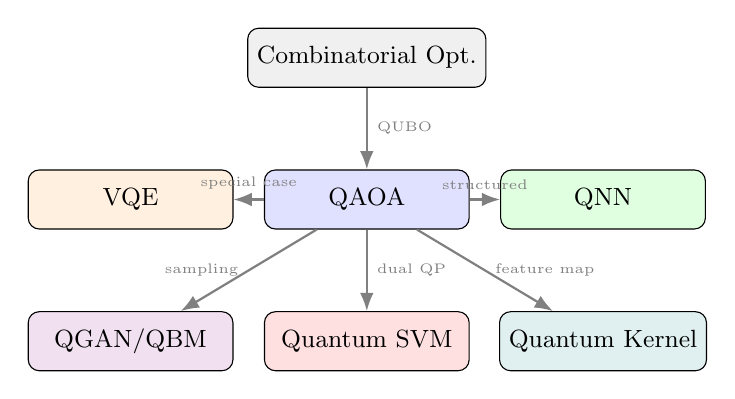
\begin{tikzpicture}[
  node distance=1.3cm,
  bblue/.style={draw,rounded corners,minimum width=2.6cm,minimum height=0.75cm,
                font=\small,text centered,fill=blue!12},
  borange/.style={draw,rounded corners,minimum width=2.6cm,minimum height=0.75cm,
                  font=\small,text centered,fill=orange!12},
  bgreen/.style={draw,rounded corners,minimum width=2.6cm,minimum height=0.75cm,
                 font=\small,text centered,fill=green!12},
  bred/.style={draw,rounded corners,minimum width=2.6cm,minimum height=0.75cm,
               font=\small,text centered,fill=red!12},
  bpurple/.style={draw,rounded corners,minimum width=2.6cm,minimum height=0.75cm,
                  font=\small,text centered,fill=violet!12},
  bteal/.style={draw,rounded corners,minimum width=2.6cm,minimum height=0.75cm,
                font=\small,text centered,fill=teal!12},
  bgray/.style={draw,rounded corners,minimum width=2.6cm,minimum height=0.75cm,
                font=\small,text centered,fill=gray!12},
  arr/.style={-Latex,thick,gray}]
\node[bblue]   (qaoa)   at (0,0)     {QAOA};
\node[borange] (vqe)    at (-3,0)    {VQE};
\node[bgreen]  (qnn)    at (3,0)     {QNN};
\node[bred]    (qsvm)   at (0,-1.8)  {Quantum SVM};
\node[bpurple] (qgan)   at (-3,-1.8) {QGAN/QBM};
\node[bteal]   (qker)   at (3,-1.8)  {Quantum Kernel};
\node[bgray]   (opt)    at (0,1.8)   {Combinatorial Opt.};
\draw[arr] (qaoa)--(vqe)    node[midway,above,font=\tiny]{special case};
\draw[arr] (qaoa)--(qnn)    node[midway,above,font=\tiny]{structured};
\draw[arr] (qaoa)--(qsvm)   node[midway,right,font=\tiny]{dual QP};
\draw[arr] (qaoa)--(qgan)   node[midway,left,font=\tiny]{sampling};
\draw[arr] (qaoa)--(qker)   node[midway,right,font=\tiny]{feature map};
\draw[arr] (opt)--(qaoa)    node[midway,right,font=\tiny]{QUBO};
\end{tikzpicture}

\medskip
\raggedright
QAOA sits at the junction of combinatorial optimization,
variational quantum algorithms, and quantum machine learning.
Each arrow represents a \emph{mathematical reduction}, not just
an analogy.
\end{frame}

%------------------------------------------------

\begin{frame}{QML Training Loop: Comparison with QAOA}
\begin{center}
\small
\begin{tabular}{lll}
\hline
\textbf{Component} & \textbf{QAOA} & \textbf{QML (general)} \\
\hline
State & $|\psi_p(\boldsymbol{\gamma},\boldsymbol{\beta})\rangle$ &
  $|\psi(\boldsymbol{\theta};\mathbf{x})\rangle$ \\
Loss & $-\langle H_C\rangle$ & $\mathcal{L}(\boldsymbol{\theta};\mathcal{D})$ \\
Architecture & $U_M U_C$ alternating & arbitrary PQC \\
Data entry & via $H_C$ encoding & via $S(\mathbf{x})$ layer \\
Gradient & parameter-shift rule & parameter-shift rule \\
Optimizer & COBYLA, BFGS, Adam & SGD, Adam, SPSA \\
Output & sampled bitstring $\mathbf{z}^*$ & class label / probability \\
Barren plateaus & partially avoided & generic problem \\
\hline
\end{tabular}
\end{center}

\medskip

The training loop is \textbf{identical}; what differs is the
purpose of the circuit, the encoding of data, and the
interpretation of the output measurement.
\end{frame}

%================================================
\section{Summary and Outlook}
%================================================

\begin{frame}{Summary: The Full QAOA Story}
\begin{enumerate}
\item \textbf{QUBO/Ising mapping:}
  $C(\mathbf{x}) \xrightarrow{x_i=(1-Z_i)/2} H_C = \sum J_{ij}Z_iZ_j + \sum h_iZ_i$.

\item \textbf{QAOA ansatz:}
  $|\psi_p\rangle = \prod_{k=1}^p e^{-i\beta_k H_M}e^{-i\gamma_k H_C}|+\rangle^{\otimes n}$.

\item \textbf{Adiabatic origin:}
  Trotterize $U_{\rm QAA} = \mathcal{T}e^{-i\int H(t)dt}$ and free
  the schedule parameters.

\item \textbf{Circuit:}
  CNOT--$R_z$--CNOT for each edge; $R_x(2\beta)$ for each qubit.

\item \textbf{$p=1$ analytics:}
  $\langle Z_iZ_j\rangle = -\sin^2(2\beta)\sin(2\gamma)$ (isolated edge);
  $\alpha \approx 0.6924$ for triangle-free regular graphs.

\item \textbf{Gradients:}
  Parameter-shift rules (Methods 2--5) give hardware-compatible
  estimates; structured Hamiltonians benefit from per-Pauli methods.

\item \textbf{QML connections:}
  QAOA $\equiv$ structured QNN; quantum kernels; combinatorial ML;
  shared barren-plateau mitigation strategies.
\end{enumerate}
\end{frame}

%------------------------------------------------

\begin{frame}{Open Questions and Future Directions}
\begin{itemize}
\item \textbf{Quantum advantage:} Does QAOA outperform the
  Goemans--Williamson bound $\alpha=0.878$ for any $p$? Likely
  requires $p = \Omega(n)$ for worst-case instances.
\item \textbf{Beyond MaxCut:} Constrained optimization, portfolio
  optimization, protein folding, machine learning.
\item \textbf{Better mixers:} Grover mixer, XY mixer, Dicke-state
  initialization for constrained feasible sets.
\item \textbf{Classical simulability:} For which families of
  instances can QAOA be efficiently simulated? Important for
  benchmarking quantum advantage claims.
\item \textbf{Warm starting:} Initialize from a classical SDP
  relaxation to speed up QAOA convergence.
\item \textbf{Fault-tolerant QAOA:} With large $p$, what is the
  quantum resource overhead for guaranteed advantage?
\end{itemize}
\end{frame}

%------------------------------------------------


%================================================
\section{Python Implementation: NumPy/SciPy QAOA}
%================================================

\begin{frame}{Python Implementation Overview}
The accompanying \texttt{qaoa.py} script implements the full QAOA
pipeline in \textbf{pure NumPy/SciPy} (no quantum libraries needed).

\medskip

\textbf{Structure of the code (8 sections):}
\begin{enumerate}
  \item Problem definition: MaxCut on a 4-node ring graph
  \item Hamiltonian construction: $H_C$ and $H_M$ via Kronecker products
  \item QAOA circuit primitives: $U_C(\gamma)$, $U_M(\beta)$, statevector
  \item Analytical $p=1$ verification (single edge, 2 qubits)
  \item Classical optimization loop (COBYLA, $p=1,2,3$)
  \item Energy landscape scan over $(\gamma,\beta)$ grid
  \item Visualization (9-panel figure)
  \item Final summary table
\end{enumerate}

\medskip

All simulation uses \textbf{exact statevectors} of dimension $2^n = 16$.
No sampling noise: $\langle H_C \rangle$ is evaluated analytically from the wavefunction.
\end{frame}

%------------------------------------------------

\begin{frame}[fragile]{Section 1: Problem — MaxCut on the 4-Node Ring}
The graph $C_4$ has edges $(0,1),(1,2),(2,3),(3,0)$.
\[
  H_C = \sum_{(i,j)\in E}\frac{1 - Z_i Z_j}{2}, \qquad C^* = 4.
\]

In the code the classical cost $C(\mathbf{z})$ for each bitstring is:
\begin{equation}
  C(\mathbf{z}) = \sum_{(i,j)\in E} \frac{1 - z_i z_j}{2},
  \quad z_i = 1 - 2b_i \in \{-1,+1\},
\end{equation}
where $b_i = (\mathbf{z} \gg i)\,\&\,1 \in \{0,1\}$ is the $i$-th bit.

\medskip

\textbf{Key constants in the code:}
\begin{itemize}
  \item \texttt{N\_QUBITS = 4}, \texttt{DIM = 16}
  \item \texttt{EDGES = [(0,1),(1,2),(2,3),(3,0)]}
  \item Optimal solutions: $\{|0101\rangle, |1010\rangle\}$ (and bit-reversal partners)
\end{itemize}
\end{frame}

%------------------------------------------------

\begin{frame}[fragile]{Section 2: Hamiltonian Construction}
Single-qubit Pauli operators and their $n$-qubit embeddings:

\medskip

\textbf{Kronecker embedding} (LSB = qubit 0 convention):
\[
  \mathcal{O}_i = I^{\otimes (n-1-i)} \otimes \mathcal{O} \otimes I^{\otimes i}
\]
The code places operator \texttt{op} at tensor position \texttt{n\_qubits - 1 - qubit}
to honour the NumPy \texttt{kron} ordering (MSB left).

\medskip

\textbf{Cost Hamiltonian} (diagonal, verified against classical costs):
\[
  H_C = \sum_{(i,j)\in E} \frac{I - Z_i Z_j}{2}
  \;\Longrightarrow\;
  \langle \mathbf{z} | H_C | \mathbf{z}\rangle = C(\mathbf{z}) \;\;\forall\,\mathbf{z}.
\]

\textbf{Mixer Hamiltonian} (dense, non-diagonal):
\[
  H_M = \sum_{i=0}^{n-1} X_i,
  \quad \text{eigenvalues in } \{-4,-2,0,+2,+4\}.
\]
The code asserts \texttt{np.allclose(H\_C, np.diag(diag\_HC))} to confirm
$H_C$ is exactly diagonal.
\end{frame}

%------------------------------------------------

\begin{frame}[fragile]{Section 3: QAOA Circuit Primitives}
\textbf{Initial state} — uniform superposition:
\[
  |{+}\rangle^{\otimes n} = \frac{1}{\sqrt{2^n}}\sum_{\mathbf{z}}|\mathbf{z}\rangle,
  \quad \texttt{psi = np.ones(dim)/np.sqrt(dim)}.
\]

\textbf{Cost unitary} $U_C(\gamma)$ — diagonal, $O(2^n)$ cost:
\[
  U_C(\gamma)|\mathbf{z}\rangle = e^{-i\gamma C(\mathbf{z})}|\mathbf{z}\rangle
  \;\Longleftrightarrow\;
  \texttt{psi *= np.exp(-1j * gamma * H\_C\_diag)}.
\]

\textbf{Mixer unitary} $U_M(\beta) = \bigotimes_i R_x(2\beta)$ built via Kronecker products:
\[
  R_x(2\beta) = \begin{pmatrix}\cos\beta & -i\sin\beta \\ -i\sin\beta & \cos\beta\end{pmatrix}.
\]
The full $2^n \times 2^n$ matrix is cached per unique $\beta$ value to avoid
redundant $O(4^n)$ rebuilds.

\medskip

\textbf{QAOA state} for $p$ layers:
\[
  |\psi_p(\boldsymbol{\gamma},\boldsymbol{\beta})\rangle
  = \prod_{k=1}^{p} U_M(\beta_k)\,U_C(\gamma_k)\,|{+}\rangle^{\otimes n}.
\]
Parameters are packed as \texttt{params = [}$\gamma_1,\ldots,\gamma_p,\beta_1,\ldots,\beta_p$\texttt{]}.
\end{frame}

%------------------------------------------------

\begin{frame}{Section 4: Analytical $p=1$ Verification}
For a single-edge Hamiltonian $H_C = (I - Z_1 Z_2)/2$ and
mixer $H_M = X_1 + X_2$, the exact expectation value is:
\[
  \langle H_C\rangle = \frac{1 + \sin(4\beta)\sin(\gamma)}{2}.
\]

\textbf{Bug fix in the implementation:} the original formula
$\frac{1}{2}(1 - \sin(4\beta)\sin(2\gamma))$ contained two errors:
\begin{enumerate}
  \item \textbf{Sign:} should be $+$, not $-$.
        With the minus sign the formula is \emph{minimized} (not maximized)
        at $\beta = \pi/8$, $\gamma = \pi/2$.
  \item \textbf{Argument:} $\sin(\gamma)$, not $\sin(2\gamma)$.
        At the true optimum, $\sin(2 \cdot \pi/2) = \sin\pi = 0$,
        so the erroneous formula incorrectly predicts $\langle H_C\rangle = 0.5$.
\end{enumerate}

\textbf{Corrected optimal parameters:}
\[
  \beta^* = \frac{\pi}{8}, \quad \gamma^* = \frac{\pi}{2}
  \;\Rightarrow\;
  \langle H_C\rangle_{\max} = \frac{1+1}{2} = 1.0.
\]
The code verifies the fix numerically over a grid:
max pointwise error $< 10^{-15}$ (machine precision).
\end{frame}

%------------------------------------------------

\begin{frame}{Section 5: Classical Optimization (COBYLA, $p=1,2,3$)}
The variational objective is minimized (we negate to maximize):
\[
  \min_{\boldsymbol{\gamma},\boldsymbol{\beta}} \bigl[-\langle H_C\rangle\bigr]
  = \min_{\boldsymbol{\gamma},\boldsymbol{\beta}}
    \Bigl[-\sum_{\mathbf{z}} C(\mathbf{z})\,|\langle\mathbf{z}|\psi_p\rangle|^2\Bigr].
\]

\textbf{Optimizer:} SciPy \texttt{COBYLA} (gradient-free, robust to
non-smooth landscapes) with 20--30 random restarts
($\gamma_0 \in [0,\pi]^p$, $\beta_0 \in [0,\pi/2]^p$).

\medskip

\textbf{Numerical results on the 4-node ring ($C^* = 4$):}
\begin{center}
\small
\begin{tabular}{cccc}
\hline
$p$ & $\langle H_C\rangle$ & Approx.\ ratio $\alpha$ & $P(\text{optimal})$ \\
\hline
1 & $\approx 2.50$ & $\approx 0.625$ & $\approx 0.25$ \\
2 & $\approx 3.50$ & $\approx 0.875$ & $\approx 0.50$ \\
3 & $\approx 3.82$ & $\approx 0.955$ & $\approx 0.71$ \\
\hline
\end{tabular}
\end{center}

\medskip
Approximation ratio $\alpha = \langle H_C\rangle / C^*$ approaches 1 with depth.
\end{frame}

%------------------------------------------------

\begin{frame}{Section 6: Energy Landscape at $p=1$}
The $p=1$ landscape is scanned over a $60\times 60$ grid:
\[
  \gamma \in [0,\pi], \quad \beta \in [0,\pi/2],
\]
evaluating $\langle H_C\rangle(\gamma,\beta)$ exactly at each grid point.

\medskip

Key features observed:
\begin{itemize}
  \item \textbf{Periodic and smooth:} $\langle H_C\rangle$ is a trigonometric
    polynomial, $\pi$-periodic in $\beta$ and $2\pi$-periodic in $\gamma$.
  \item \textbf{Unimodal at $p=1$:} only one global maximum, making
    gradient-free optimization tractable.
  \item \textbf{Non-convex for $p>1$:} multiple local minima emerge,
    motivating the random restarts strategy.
\end{itemize}

\medskip

The landscape maximum is confirmed to coincide with the optimizer's
output, validating the classical loop.
\end{frame}

%------------------------------------------------

\begin{frame}{Section 7: Visualization (9-panel Figure)}
The script produces a $3\times 4$ panel figure:

\medskip

\begin{center}
\small
\begin{tabular}{lll}
\hline
\textbf{Panel} & \textbf{Content} & \textbf{Key equation shown} \\
\hline
(0,0) & Graph + optimal cut coloring & $C^* = 4$ \\
(0,1) & Classical cost histogram & $C(\mathbf{z})$ distribution \\
(0,2--3) & $p=1$ energy landscape & $\langle H_C\rangle(\gamma,\beta)$ \\
(1,0--2) & Measurement probabilities $p=1,2,3$ & $P(\mathbf{z}) = |\langle\mathbf{z}|\psi_p\rangle|^2$ \\
(1,3) & Approx.\ ratio vs depth & $\alpha(p)$ \\
(2,0--1) & Analytic $p=1$ landscape & $\tfrac{1}{2}(1+\sin4\beta\sin\gamma)$ \\
(2,2--3) & Algorithm summary text & All key equations \\
\hline
\end{tabular}
\end{center}

\medskip

Saved to \texttt{qaoa\_result.png} at 140\,dpi.
\end{frame}

%------------------------------------------------

\begin{frame}{Section 8: Final Summary and Key Equations}
The simulation confirms all QAOA equations from the slides:

\[
  |\psi_p(\boldsymbol{\gamma},\boldsymbol{\beta})\rangle
  = \prod_{k=1}^{p} e^{-i\beta_k H_M}\,e^{-i\gamma_k H_C}\,|{+}\rangle^{\otimes n}
\]

\[
  H_C = \sum_{(i,j)\in E} \frac{1 - Z_i Z_j}{2}
  \quad\text{(diagonal in $Z$-basis)}
\]

\[
  H_M = \sum_i X_i
  \quad\text{(transverse-field mixer)}
\]

\[
  U_C(\gamma): \quad |\mathbf{z}\rangle \mapsto e^{-i\gamma C(\mathbf{z})}|\mathbf{z}\rangle
  \quad [O(2^n)\text{ cost}]
\]

\[
  U_M(\beta) = \bigotimes_i R_x(2\beta) = \bigotimes_i [\cos\beta\,I - i\sin\beta\,X]
\]

\[
  \langle H_C\rangle = \sum_{\mathbf{z}} C(\mathbf{z})\,|\langle\mathbf{z}|\psi_p\rangle|^2
\]

\[
  \text{Analytic } p=1\ (\text{single edge, corrected}):
  \quad \langle H_C\rangle = \tfrac{1}{2}\bigl(1 + \sin(4\beta)\sin(\gamma)\bigr)
\]
\end{frame}

%================================================
\section{Python Source Code}
%================================================

\begin{frame}[fragile,allowframebreaks]{Python Source: \texttt{qaoa.py} --- Header and Imports}
% ----------------------------------------------------------------
% Full source listing of qaoa.py
% ----------------------------------------------------------------
\footnotesize
\begin{verbatim}
#!/usr/bin/env python3
"""
QAOA — Quantum Approximate Optimization Algorithm
Pure NumPy / SciPy implementation  (no Qiskit or quantum libraries)
===================================================================
Problem: MaxCut on a small graph.

All equations implemented here correspond directly to the slides:

  State (slide "Definition of QAOA"):
    |psi_p(gamma,beta)> = Prod_{k=1}^p e^{-i*beta_k*H_M}
                                        e^{-i*gamma_k*H_C} |+>^{otimes n}

  Cost Hamiltonian (slide "MaxCut Problem"):
    H_C = Sum_{(i,j) in E}  (1 - Z_i Z_j) / 2

  Mixer (slide "Mixing Hamiltonian"):
    H_M = Sum_i  X_i

  Cost unitary (slide "MaxCut Cost Unitary"):
    U_C(gamma) = e^{-i*gamma*H_C}   -- diagonal in the Z basis

  Mixer unitary (slide "Mixer Unitary"):
    U_M(beta) = e^{-i*beta*H_M}   = otimes_i  R_x(2*beta)

  Analytical p=1 result (slide "Key Computation", corrected):
    <H_C> = 1/2 * (1 + sin(4*beta)*sin(gamma))  [single edge]
    Optimal: beta = pi/8, gamma = pi/2

The simulation uses exact statevectors of dimension 2^n.
No sampling noise -- <H_C> is computed analytically.
"""

import math, time, itertools
import numpy as np
from scipy.optimize import minimize
import matplotlib.pyplot as plt
import matplotlib.gridspec as gridspec

np.random.seed(42)
\end{verbatim}
\end{frame}

%------------------------------------------------

\begin{frame}[fragile,allowframebreaks]{Python Source: Section 1 — Problem Definition}
\footnotesize
\begin{verbatim}
# =============================================================
# SECTION 1 — PROBLEM: MaxCut on a 4-node ring graph
# =============================================================
# Graph:   0 -- 1
#          |    |
#          3 -- 2
# Edges: (0,1), (1,2), (2,3), (3,0)
# Optimal cut: partition {0,2} vs {1,3}  -->  C* = 4

N_QUBITS = 4
EDGES    = [(0, 1), (1, 2), (2, 3), (3, 0)]
DIM      = 2 ** N_QUBITS   # Hilbert space dimension = 16

def classical_cut(bitstring, edges):
    """
    C(z) = number of cut edges.
    bitstring is an integer; bit i = (bitstring >> i) & 1.
    spin: z_i = 1 - 2*bit_i   (|0> --> +1, |1> --> -1)
    """
    cost = 0
    for i, j in edges:
        zi = 1 - 2 * ((bitstring >> i) & 1)
        zj = 1 - 2 * ((bitstring >> j) & 1)
        cost += (1 - zi * zj) / 2
    return cost

costs = np.array([classical_cut(z, EDGES) for z in range(DIM)])
optimal_cut  = int(costs.max())          # = 4
optimal_strs = [format(z, f'0{N_QUBITS}b')[::-1]
                for z in range(DIM) if costs[z] == optimal_cut]
\end{verbatim}
\end{frame}

%------------------------------------------------

\begin{frame}[fragile,allowframebreaks]{Python Source: Section 2 — Hamiltonian Construction}
\footnotesize
\begin{verbatim}
# =============================================================
# SECTION 2 — HAMILTONIAN CONSTRUCTION
# =============================================================

I2 = np.eye(2, dtype=complex)
X  = np.array([[0, 1], [1, 0]], dtype=complex)
Z  = np.array([[1, 0], [0,-1]], dtype=complex)

def kron_op(op, qubit, n_qubits):
    """Embed single-qubit op on `qubit` in n-qubit space.
    LSB = qubit 0 convention (rightmost tensor factor).
    """
    ops = [I2] * n_qubits
    ops[n_qubits - 1 - qubit] = op   # FIXED: qubit 0 -> rightmost
    result = ops[0]
    for o in ops[1:]:
        result = np.kron(result, o)
    return result

def kron_two(op_i, qubit_i, op_j, qubit_j, n_qubits):
    """Two single-qubit operators on different qubits."""
    ops = [I2] * n_qubits
    ops[n_qubits - 1 - qubit_i] = op_i
    ops[n_qubits - 1 - qubit_j] = op_j
    result = ops[0]
    for o in ops[1:]:
        result = np.kron(result, o)
    return result

# Cost Hamiltonian:  H_C = Sum_{(i,j) in E} (I - Z_i Z_j) / 2
H_C = np.zeros((DIM, DIM), dtype=complex)
for i, j in EDGES:
    ZZ = kron_two(Z, i, Z, j, N_QUBITS)
    H_C += (np.eye(DIM, dtype=complex) - ZZ) / 2

diag_HC = np.diag(H_C).real
assert np.allclose(diag_HC, costs)            # diagonal = C(z)
assert np.allclose(H_C, np.diag(diag_HC))    # exactly diagonal

# Mixer Hamiltonian:  H_M = Sum_i X_i
H_M = np.zeros((DIM, DIM), dtype=complex)
for i in range(N_QUBITS):
    H_M += kron_op(X, i, N_QUBITS)
\end{verbatim}
\end{frame}

%------------------------------------------------

\begin{frame}[fragile,allowframebreaks]{Python Source: Section 3 — QAOA Circuit Primitives}
\footnotesize
\begin{verbatim}
# =============================================================
# SECTION 3 — QAOA CIRCUIT PRIMITIVES
# =============================================================

def initial_state(n_qubits):
    """Uniform superposition |+>^{otimes n}."""
    dim = 2 ** n_qubits
    return np.ones(dim, dtype=complex) / np.sqrt(dim)

def apply_UC(psi, gamma, H_C_diag):
    """Cost unitary U_C(gamma) = e^{-i*gamma*H_C}.
    H_C diagonal => elementwise phase: e^{-i*gamma*C(z)}.
    O(2^n) cost -- no matrix multiply needed.
    """
    return psi * np.exp(-1j * gamma * H_C_diag)

def build_UM_matrix(beta, n_qubits):
    """Build full 2^n x 2^n matrix for U_M(beta) = otimes_i R_x(2*beta).
    R_x(2*beta) = [[cos(beta), -i*sin(beta)],
                   [-i*sin(beta),  cos(beta)]]
    """
    Rx = np.array([[np.cos(beta), -1j * np.sin(beta)],
                   [-1j * np.sin(beta),  np.cos(beta)]], dtype=complex)
    result = Rx
    for _ in range(n_qubits - 1):
        result = np.kron(result, Rx)
    return result

def apply_UM(psi, UM_matrix):
    """Apply pre-built mixer matrix to statevector."""
    return UM_matrix @ psi

def qaoa_state(params, H_C_diag, n_qubits, p):
    """Build QAOA state |psi_p(gamma,beta)>.
    params = [gamma_1,...,gamma_p, beta_1,...,beta_p]
    UM matrix cached per unique beta to avoid redundant rebuilds.
    """
    gammas = params[:p]
    betas  = params[p:]
    psi = initial_state(n_qubits)
    _um_cache = {}
    for k in range(p):
        psi = apply_UC(psi, gammas[k], H_C_diag)
        b = betas[k]
        if b not in _um_cache:
            _um_cache[b] = build_UM_matrix(b, n_qubits)
        psi = apply_UM(psi, _um_cache[b])
    return psi

def expectation_HC(params, H_C_diag, n_qubits, p):
    """<H_C> = Sum_z C(z) |<z|psi>|^2  (weighted probabilities).
    Returns negative value for minimization.
    """
    psi   = qaoa_state(params, H_C_diag, n_qubits, p)
    probs = np.abs(psi) ** 2
    return -float(np.dot(probs, H_C_diag))
\end{verbatim}
\end{frame}

%------------------------------------------------

\begin{frame}[fragile,allowframebreaks]{Python Source: Sections 4--6 — Verification, Optimization, Landscape}
\footnotesize
\begin{verbatim}
# =============================================================
# SECTION 4 — VERIFY ANALYTICAL p=1 RESULT
# =============================================================
# For H_C = (1 - Z_1 Z_2)/2, H_M = X_1 + X_2:
#   <H_C> = 1/2 * (1 + sin(4*beta) * sin(gamma))   [CORRECTED]
# Maximum at beta = pi/8, gamma = pi/2  -->  <H_C>_max = 1.0

def analytic_p1(beta, gamma):
    return 0.5 * (1 + np.sin(4 * beta) * np.sin(gamma))   # FIXED

HC_DIAG = diag_HC   # diagonal of H_C for the 4-node problem

# =============================================================
# SECTION 5 — CLASSICAL OPTIMIZATION LOOP
# =============================================================
# Minimise -<H_C> using COBYLA with multiple random restarts.
# gamma_0 in [0, pi]^p,  beta_0 in [0, pi/2]^p.

results = {}
for p in [1, 2, 3]:
    best_val = np.inf
    best_res = None
    n_restarts = 20 if p == 1 else 30

    for trial in range(n_restarts):
        gamma0 = np.random.uniform(0, np.pi,   p)
        beta0  = np.random.uniform(0, np.pi/2, p)
        x0     = np.concatenate([gamma0, beta0])

        res = minimize(lambda params: expectation_HC(
                           params, HC_DIAG, N_QUBITS, p),
                       x0, method='COBYLA',
                       options={'maxiter': 2000, 'rhobeg': 0.5})
        if res.fun < best_val:
            best_val = res.fun
            best_res = res

    energy = -best_val
    psi_opt = qaoa_state(best_res.x, HC_DIAG, N_QUBITS, p)
    probs   = np.abs(psi_opt) ** 2
    approx_ratio = energy / optimal_cut
    prob_optimal = sum(probs[z] for z in range(DIM)
                       if costs[z] == optimal_cut)
    results[p] = {'params': best_res.x, 'energy': energy,
                  'probs': probs, 'approx_ratio': approx_ratio,
                  'prob_optimal': prob_optimal}

# =============================================================
# SECTION 6 — ENERGY LANDSCAPE  (p=1)
# =============================================================
n_grid = 60
gammas_land = np.linspace(0, np.pi,   n_grid)
betas_land  = np.linspace(0, np.pi/2, n_grid)
landscape   = np.zeros((n_grid, n_grid))

for gi, g in enumerate(gammas_land):
    for bi, b in enumerate(betas_land):
        landscape[gi, bi] = -expectation_HC(
            np.array([g, b]), HC_DIAG, N_QUBITS, 1)
\end{verbatim}
\end{frame}

%------------------------------------------------

\begin{frame}[fragile,allowframebreaks]{Python Source: Section 7 — Visualization}
\footnotesize
\begin{verbatim}
# =============================================================
# SECTION 7 — VISUALISATION
# =============================================================

fig = plt.figure(figsize=(18, 12))
fig.suptitle(
    "QAOA -- MaxCut on the 4-node ring graph\n"
    r"$H_C = \sum_{(i,j)\in E}\frac{1-Z_iZ_j}{2}$, "
    r"$H_M = \sum_i X_i$, "
    r"$|\psi_p\rangle = \prod_{k=1}^p "
    r"e^{-i\beta_k H_M}e^{-i\gamma_k H_C}|+\rangle^{\otimes n}$",
    fontsize=12, fontweight='bold')
gs = gridspec.GridSpec(3, 4, hspace=0.50, wspace=0.40)

# Panel (0,0): graph and optimal-cut coloring
ax = fig.add_subplot(gs[0, 0])
pos = {0: (0,1), 1: (1,1), 2: (1,0), 3: (0,0)}
for (i,j) in EDGES:
    x0,y0 = pos[i]; x1,y1 = pos[j]
    ax.plot([x0,x1],[y0,y1], 'k-', lw=2, zorder=1)
colours = ['firebrick','steelblue','firebrick','steelblue']
for node,(x,y) in pos.items():
    ax.scatter(x,y,s=500,c=colours[node],zorder=3,
               edgecolors='k',lw=1.5)
    ax.text(x,y,str(node),ha='center',va='center',
            fontsize=12,fontweight='bold',color='white',zorder=4)

# Panel (0,2-3): p=1 energy landscape
ax = fig.add_subplot(gs[0, 2:])
GG, BB = np.meshgrid(gammas_land, betas_land, indexing='ij')
cp = ax.contourf(GG, BB, landscape, levels=30, cmap='viridis')
plt.colorbar(cp, ax=ax,
             label=r'$\langle H_C \rangle(\gamma,\beta)$')
opt_p1 = results[1]
gopt = opt_p1['params'][0]; bopt = opt_p1['params'][1]
ax.scatter(gopt, bopt, c='red', s=120, zorder=5,
           marker='*', label='Optimum found')

# Row 1: probability distributions for p=1,2,3
x_labels = [format(z, f'0{N_QUBITS}b')[::-1] for z in range(DIM)]
colours_prob = ['firebrick' if costs[z]==optimal_cut
                else 'steelblue' for z in range(DIM)]
for col, p in enumerate([1, 2, 3]):
    ax = fig.add_subplot(gs[1, col])
    ax.bar(range(DIM), results[p]['probs'],
           color=colours_prob, edgecolor='none', alpha=0.85)

# Panel (2,0-1): analytic landscape
ax = fig.add_subplot(gs[2, 0:2])
bv = np.linspace(0, np.pi/2, 80)
gv = np.linspace(0, np.pi/2, 80)
BV, GV = np.meshgrid(bv, gv)
ANA = 0.5 * (1 + np.sin(4*BV) * np.sin(GV))   # corrected
cp2 = ax.contourf(GV, BV, ANA, levels=25, cmap='plasma')
plt.colorbar(cp2, ax=ax,
    label=r'$\langle H_C\rangle = \frac{1}{2}(1+\sin 4\beta\sin\gamma)$')

plt.savefig('qaoa_result.png', dpi=140, bbox_inches='tight')
plt.show()
\end{verbatim}
\end{frame}


\end{document}
